\chapter{Exploring Temporal Relationship through User Annotations}

\graphicspath{{Chapter3/figures/}}

%Timeline visualization is an important tool for sensemaking. It allows analysts to examine information in chronological order and to identify temporal patterns and relationships. However, many existing timeline visualization methods are not designed for the dynamic and iterative nature of the sensemaking process and the various analysis activities it involves. In this chapter, we introduce a novel timeline visualization, SchemaLine, to address these deficiencies.
%
%\section{Introduction}
%The importance of timeline visualization in supporting sensemaking.
%
%The current limitation
%\begin{itemize}
%	\item no or very simple layout which is cluttered and space-inefficient
%	\item designed for presenting a known story rather than interactively constructing a hidden one
%\end{itemize}  
%
%The contribution
%\begin{itemize}
%	\item a novel  design for an interactive timeline that groups notes into schema determined by the analyst,
%	\item an algorithm to automatically generate a compact and aesthetically pleasing visualization of these schema on the timeline, and
%	\item a set of fluid interactions with the timeline to support the sensemaking activities defined in the Data-Frame model.
%\end{itemize}
%
%\section{Requirements}
%[not in the paper yet! List requirements that SchemaLine need to support including the ability to sensemaking activities from Data--frame model]
%
%\section{Visual Design}
%Visual representation of individual events and schemas
%
%
%\begin{figure}[ht]
%	\centering
%	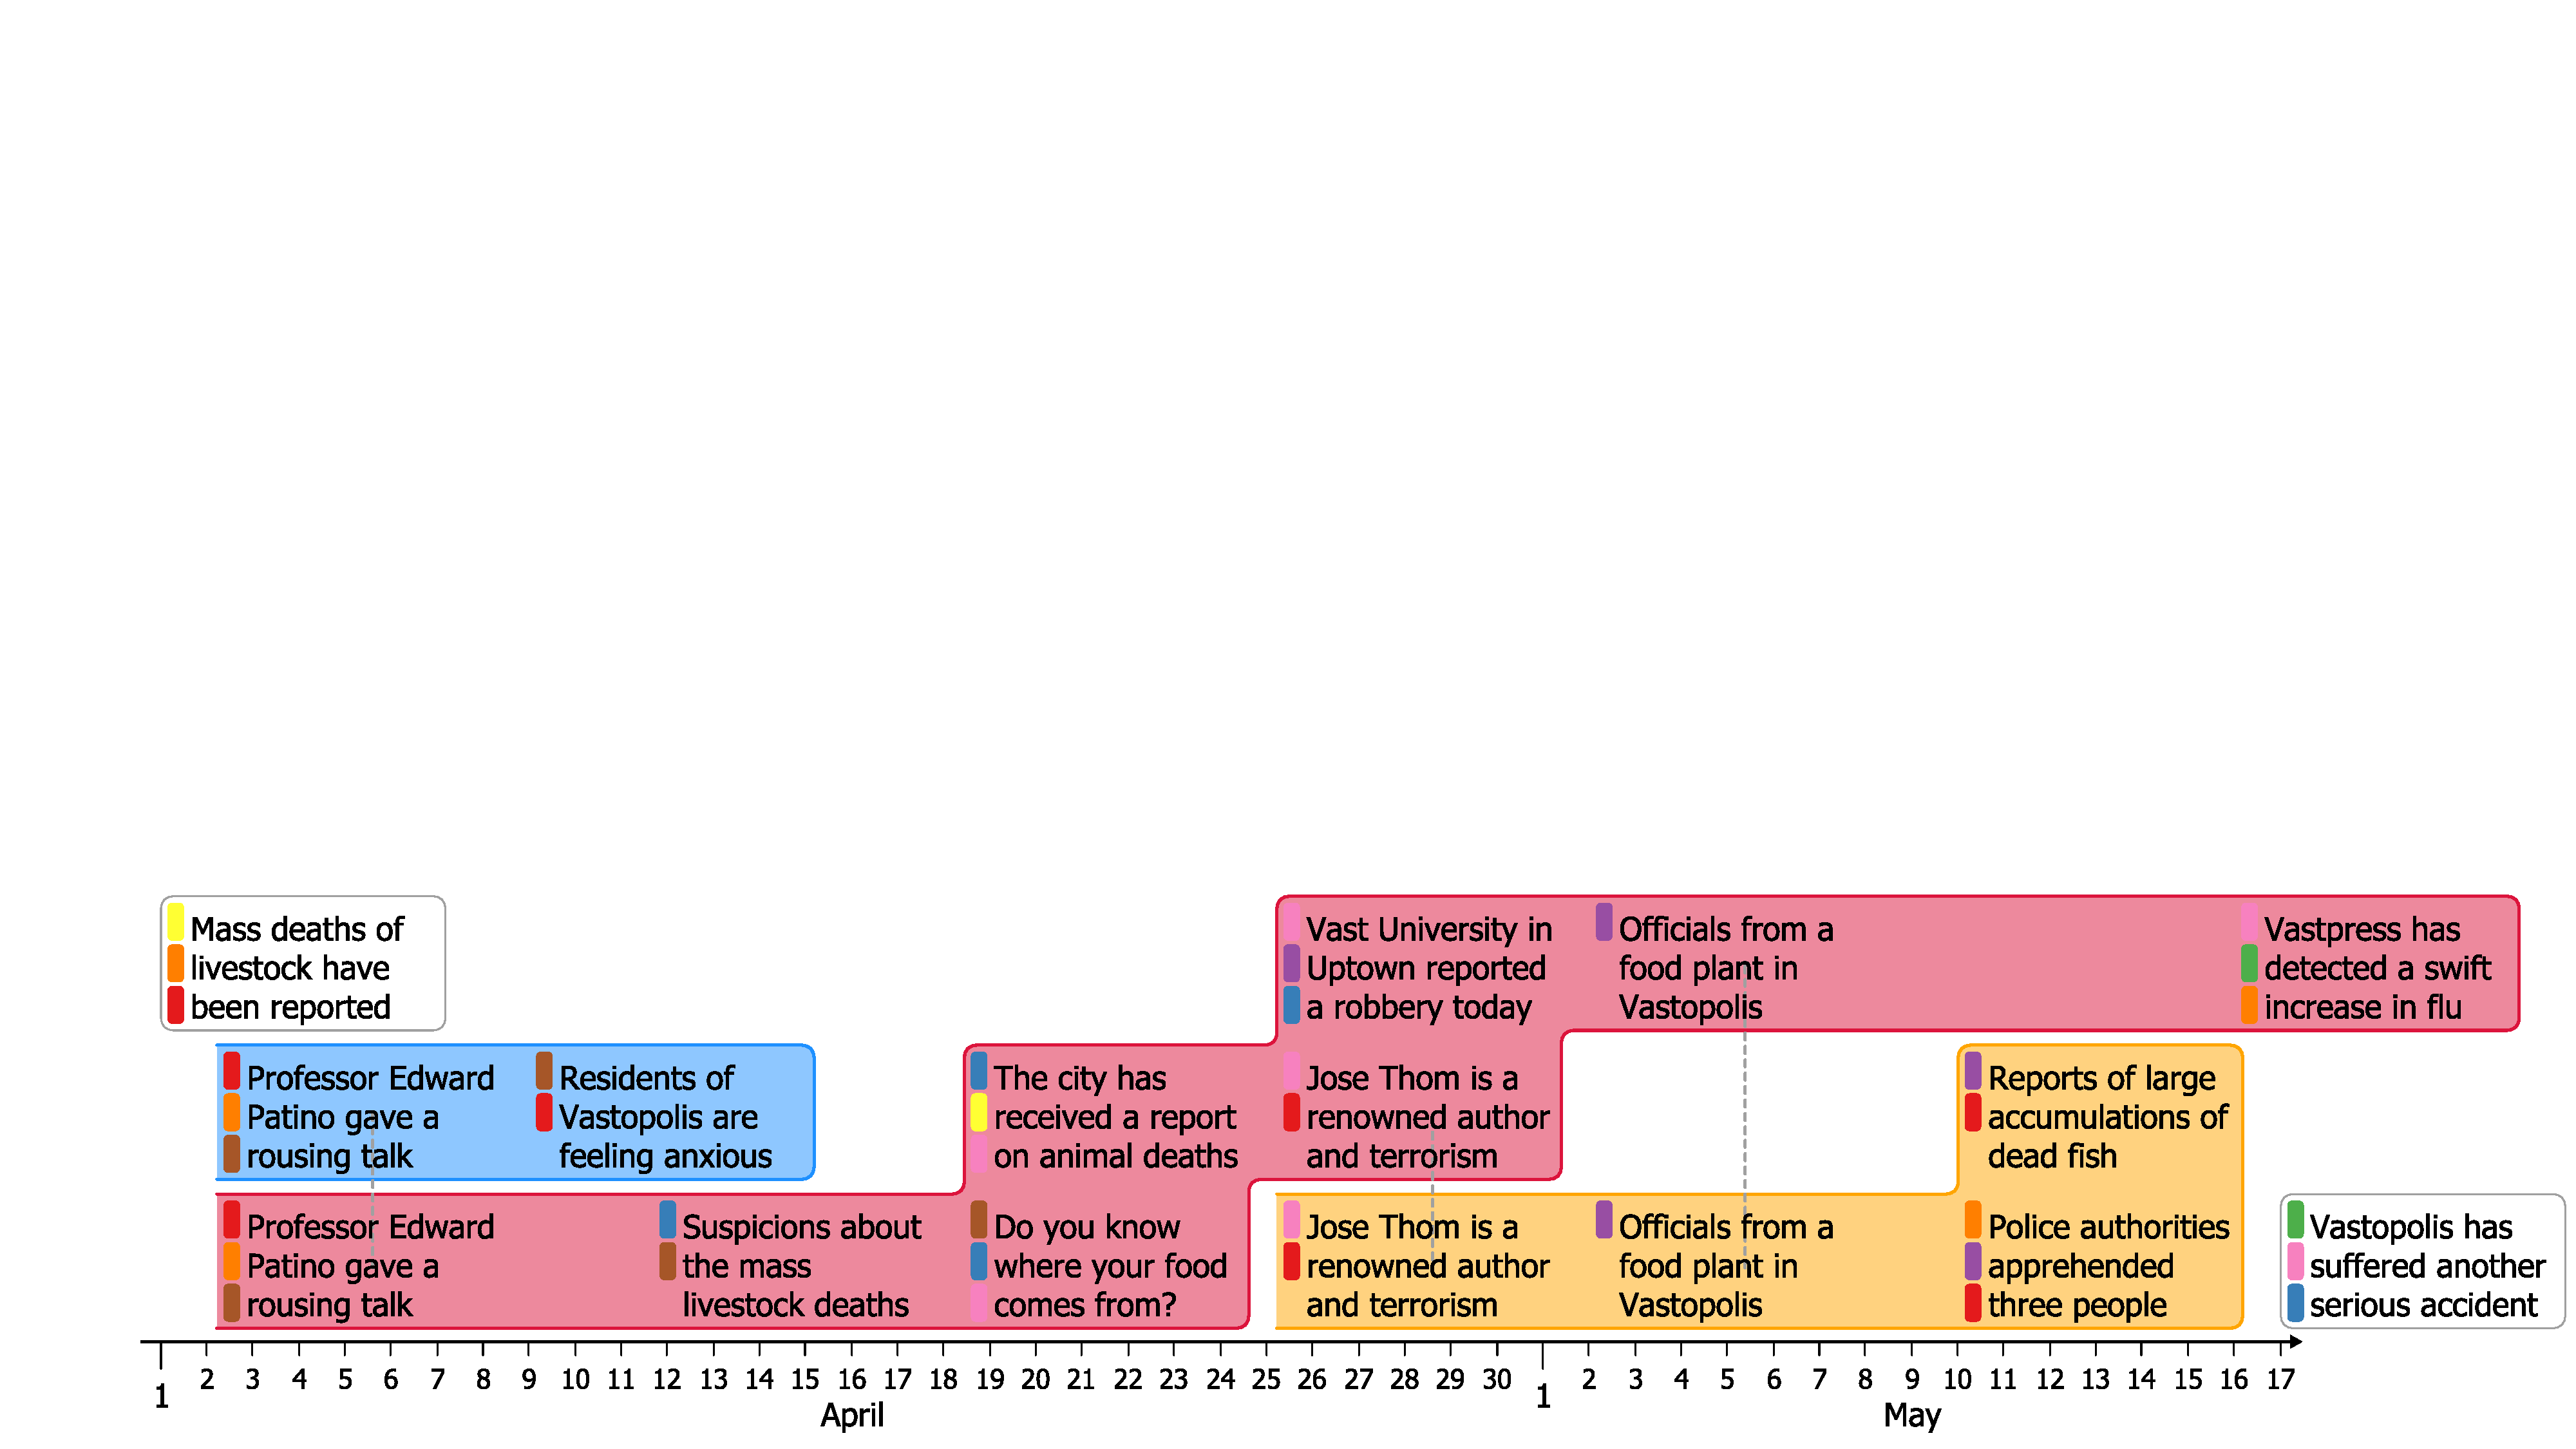
\includegraphics[width=\linewidth]{teaser}
%	\caption{SchemaLine: each piece of text is an analyst note, positioned along the time axis at when the event happened. Related notes are linked together to form a ``schema'' or ``frame''. There are three frames in this example represented as colored rectilinear paths. Small color-coded rectangles on the left side of notes are ``categories''.}
%	\label{fig:teaser}
%\end{figure}
%
%\section{Algorithm}
%
%%\subsection{Layout}
%Describe the algorithm that produces the compact layout of schemas and events.
%
%%\subsection{Schema Outline}
%%Describe the algorithm that produces the polygonal outline covering all events within a schema.
%
%%\section{Sensemaking with SchemaLine}
%%Discuss how SchemaLine's interactions support sensemaking activities in the Data--frame model. [the requirement for this support should be mentioned in the Requirements section.]
%
%\section{Application}
%Discuss the integration of SchemaLine into INVISQUE. SchemaLine receives data input as user notes of INVISQUE and the linking between schemas and index-cards.
%
%\section{Evaluation}
%A case study with 3 participants (different backgrounds) to use INVISQUE+SchemaLine to solve an intelligence analysis task using VAST Challenge 2011 dataset. Report how they used the tool, how the tool might help them.
%
%\section{Conclusion}


%\section{Introduction}
Intelligence analysis is defined as ``the application of individual and collective cognitive methods to weigh data and test hypotheses within a secret socio-cultural context''~\cite{Johnston2005}. To gain a deeper understanding into the sensemaking process in intelligence analysis, Pirolli and Card~\cite{Pirolli2005} conducted a cognitive task analysis with analysts and proposed a process model of sensemaking, which was described earlier in detail in \autoref{sub:lr-sensemaking}. During the sensemaking process, analysts need to read thousands of reports and extract relevant details, organize them in a way that help the analysts to identify patterns and generate hypotheses. This is challenging because of the large number of documents involved and the complex relationship of entities discovered. Visual analytics systems~\cite{Pioch2006,Wright2006,Stasko2007} facilitate intelligence analysis with automated techniques applied to leverage manual investigation of a large document collection. For instance, named-entity recognition techniques~\cite{Nadeau2007} can identify entities (i.e., persons, organizations and locations), and topic modeling techniques~\cite{Blei2003} can extract the main themes discussed. To help analysts manage a large number of discoveries they made during the sensemaking process, the systems allow them to externalize their thoughts through note taking. Analysts are then often supported to freely organized their notes in a way that makes sense to them and facilitates their analyses, such as constructing a timeline of suspicious events.

% Problem of exisiting timelines in sensemaking
\emph{Timeline} is a simple yet powerful technique to visualize time-oriented data~\cite{Tufte1983}, allowing exploration and identification of temporal patterns and relationships in the data. It displays events along the time axis and position them at the time points at which they occur or the time ranges over which they last~\cite{Plaisant1996}. Timelines have been applied extensively in visualizing both raw data and analysis findings for supporting sensemaking. POLESTAR~\cite{Pioch2006} and HARVEST~\cite{Gotz2006} allow analysts to take notes, define new knowledge, and explore them through a timeline visualization. Jigsaw~\cite{Gorg2013} uses timelines to organize extracted named entities, one for each type. Similarly, nSpace2 Sandbox~\cite{SandboxTimeline2012} provides the creation of multiple sub-timelines for visualizing different types of artifacts. However, these timeline visualizations either lack an automatic layout~\cite{Pioch2006} or use an overly-simplistic linear layout~\cite{SandboxTimeline2012}. As a result, the visualization requires significant effort from analysts to manually arrange data elements, making it difficult to detect temporal patterns.

Sensemaking includes dynamic activities centering around the collected data and its explanation~\cite{Klein2003}. Therefore, to support the dynamic nature of sensemaking, timeline visualizations should allow analysts to create and edit temporal structures interactively. Also, the interaction should be intuitive and fluid~\cite{Elmqvist2011} to prevent analysts from extra cognitive effort and distraction. However, existing timeline visualization techniques are mainly designed for presenting a known story rather than revealing and constructing a hidden one interactively.

In this chapter, we introduce a novel timeline visualization -- SchemaLine -- to address the aforementioned issues. More specifically, SchemaLine contributes
\begin{itemize}
	\item A visual design for an interactive timeline that groups annotations into user-determined schemas.
	\item A compact and aesthetically pleasing timeline layout.
	\item A set of fluid interactions with the timeline to support the sensemaking activities described in the Data--Frame model~\cite{Klein2003}.
\end{itemize}
%%\section{Related Work}
\label{sec:relatedwork}

%\subsection{Timeline Visualization}
% Timeline visualization
%Timeline is one of the earliest visualizations. Back in 1765, Joseph Priestley created the Chart of Biography about two thousand famous people from 1200 B.C to 1750 A.D~\cite{Priestley1765} -- one of the oldest documented timeline. Along a horizontal timeline, Priestley used bars to depict lifespans and dots to illustrate the uncertain birth and dead dates. This remains one of the most popular visual metaphors for timeline visualization: time is represented as a horizontal axis; an event is plotted as a point if it is an instant or a bar spans its interval otherwise. Geographical information can also be included in timeline visualizations as in the classic information visualization example of Napoleon's March on Moscow in 1812-1813 by Charles Joseph Minard~\cite{Minard1869}. 

In this section, we consider related work on representing temporal data and producing timelines, before also examining larger visual analytic systems that include timelines in their feature set.

\subsection{Timeline Visualizations}
% Some examples based on timeline metaphor. Aggregate methods.
A typical example of timeline visualizations is LifeLines~\cite{Plaisant1996a}, a visualization for personal histories, which uses icons to indicate discrete events and thick horizontal lines for continuous ones. When the number of data items is large, they need to be shown collectively rather than individually. The river metaphor~\cite{Havre2002} is one such method that represents thematic changes in large document collections. Storyline visualizations illustrate the dynamic relationships between entities in a story. The technique was first introduced by Munroe with his hand-drawn visualizations~\cite{Munroe2009}. The visualization summarizes movie plots by depicting each character as a line and each interaction between characters as a converging or diverging bundle of those character lines. Computational layouts have since been introduced to automate the rendering process including work by Tanahashi and Ma~\cite{Tanahashi2012} and Liu et al.~\cite{Liu2013}. 

%There are other metaphors to represent temporal data such as the three-dimensional histogram~\cite{Kosara2004}, the spiral graph~\cite{Weber2001}, or calendar-based approaches~\cite{VanWijk1999}. More detail about timelines or more general time-oriented data visualizations can be found in the comprehensive work of Aigner et al.~\cite{Aigner2011}.

% Skip scalability issue because it's not addressed in SchemaLine
%While the time axis metaphor is simple and intuitive, it can be challenging to visualize a large number of events and the relationships among them along a timeline. In the simplest case, all events are unrelated and visualized independently on the timeline. When several events happened during a short period, multiple layers above the timeline need to created to ensure each event's position matches its time point and no two event descriptions overlap~\cite{Plaisant1998,Pioch2006,Andre2007,Liu2010,Kim2010,Munroe2013,SimileTimeline,TimeGlider}. \note[k]{We mentioned timeline scalability here and need to discuss it for SchemaLine} The resulting timeline can quickly get cluttered as events and layers increase. Several attempts have been made to address the scalability issue including semantics zooming with different levels of detail \cite{Andre2007}, focus and context views \cite{Andre2007, SimileTimeline}, and aggregation of multiple events to one single event \cite{Plaisant1998}.

% Visualize relationships between events
Visualizing individual events on a timeline is relatively simple; however, showing relationships between events is quite challenging. One approach is to explicitly draw an edge between two related entities as in tmViewer~\cite{Kumar1998}. Edge styles can be used to depict different kinds of relationships; however, drawing a node-link diagram on top of the timeline can cause the visualization to become cluttered even with a small number of events. Another method is to use the concurrent perception ability of humans by using color coding or icons to indicate different groupings. When events are distributed along the timeline, this method introduces a heavy cognitive load for viewers to scan through the entire timespan. Our method uses colored backgrounds and clusters all events belonging to the same group to reduce user effort. Relationships within multiple faceted temporal data are addressed by Andr\'{e} et al. in Continuum~\cite{Andre2007} by using views with different scales and the classic details-on-demand technique to save space. More recently, SemaTime~\cite{Stab2010} can visualize two different types of relationship: time-dependent (e.g., lives-in) and time-independent (e.g., father-of). SemaTime stacks events vertically and places related events close together. Time-dependent relationships are depicted by using rectangles crossing the relevant common interval of the two events. Time-independent relationships are illustrated by simple arrows.

% Follow events in timeline
%One essential requirement in timeline visualizations is to be able to follow events chronologically. Even though events are aligned with their time, it can still be difficult to trace which events happen after which, especially when they are close. A conventional rule is that an event is preferentially rendered at the bottom. If the representation of the event (normally a short summary of the event) does not overlap with other event representations, it will stay at the bottom; otherwise, it needs to move up a level. In place of this implicit rule, our method creates an explicit path to guide readers, to improve performance in both time and accuracy. 

%Visual attributes, such as colors and font sizes, are commonly used when events have other attributes (such as grouping and importance level) need to be included in the visualization \cite{TimeGlider}. \note[k]{Similarly, we mentioned number of distinguishable colour issue here and need to discuss it for SchemaLine} However, the number of colors that can be easily distinguished is limited, and so are the levels of possible font sizes to ensure legibility and not taking up too much display estate. 

%To address these problems, LifeLines \cite{Plaisant1998} divides the vertical dimension of timeline into multiple stacks, each to represent a group of events. Continuum \cite{Andre2007} represents the hierarchical relationships between events by displaying child events nested in a parent event. For example, in the music context, a piece belongs to a composer, a composer then lives in an era. All pieces of one composer can be displayed inside a bar of the composer, which represents his/her lifespan.

%Events can have additional complex relationships. In genealogical data, there are relationships such as marriage/divorce and parent-child. \note[k]{can reduce the details about this work if need space}{Kim et al. \cite{Kim2010} represent people as individual lines that cover their lifespans. Vertical axis is used to represent relationships. Unrelated people are displayed vertically far enough to indicate that there is no relationship between them. When two persons get married, the two corresponding lines converge into a bundle to indicate a marriage. Whereas, the diverge of a bundle of two lines denote a divorce. The child is visualized close to the bundle of his parents and a vertical faded dash-line is used to connect the beginning of the child line to his parents.} 

%Another example is movie data, in which a scene contains a start time, a duration and members involved. Munroe creates a hand-drawn visualization to summarize characters' interactions in movies, published in the XKCD webcomic ``Movie Narrative Charts'' \cite{Munroe2013}. Inspired from that work, Tanahashi and Ma~\cite{Tanahashi2012} propose a set of design considerations for aesthetic and legible story-line visualizations, and an algorithm to generate visualizations satisfying these design principles. Similar to representing marriage/divorce relationship in genealogical data,  character lines should go straight unless they converge to or diverge from an interaction. The bundle of lines in an interaction should be adjacent; otherwise, lines must be not adjacent to depict separate character lines. To improve the aesthetics and legibility of the visualization, the algorithm also tries to minimize the number of line wiggles (bends), line crossovers, and white space gaps. The visual representation of SchemaLine is inspired by this work. 

%\subsection{Narrative Construction}
%\label{sec:narrative}
%Segel and Heer \cite{Segel2010} reviewed and classified narrative visualizations based on three dimensions: genre, visual narrative tactics, and narrative structure tactics. They define seven (not mutually exclusive) genres of narrative visualizations including magazine style, annotated chart, partitioned poster, flow chart, comic strip, live show, and film/video/animation. Narrative visualizations can also be classified as author-driven, reader-driven, or hybrid. They give an example of a common approach called "Martini Glass Structure". The story begins with the author's guidance for a while and then leads to the reader-driven stage where they can freely explore the story. Among these, most relevant to our work are those designed for sensemaking and utilize a timeline representation.

\subsection{Timelines within Visual Analytics Systems}
A timeline is commonly integrated into Visual Analytics systems designed for making sense of large and complex datasets including POLESTAR~\cite{Pioch2006}, HARVEST~\cite{Gotz2006}, Jigsaw~\cite{Stasko2007, Gorg2013}, and nSpace2 Sandbox~\cite{Wright2006, SandboxTimeline2012}. 

% visualize what?
To support sensemaking, timelines are typically used to visualize not raw data, but more meaningful information such as user notes (POLESTAR, HARVEST) or extracted entities (Jigsaw, nSpace2 Sandbox) instead. HARVEST visualizes both raw data and synthesized knowledge in one timeline to allow progressive investigation. However, filtering must be supported to prevent valuable information getting lost among dense data.

% manipulation of notes
Most of the systems use timelines to show notes statically, to present a known story instead of dynamically discovering a hidden story. nSpace2 Sandbox is an exception -- it allows users to group related entities into sub-timelines and to alter the entity's date on the timeline if needed. However, one entity cannot be added into multiple timelines, which is necessary when an entity's category is uncertain. Our SchemaLine provides a set of fluid interactions to manipulate notes to build a more semantic schema.

% visual representation of notes and schemata
Notes are typically represented using the ``sticky-notes'' metaphor: a colored rectangle as background with text on top of it. nSpace2 Sandbox provides multiple levels of detail for entities: a short summary, a full article, or even entities of entities. Timelines are commonly visualized as a horizontal axis with notes connecting to the timeline by edges. nSpace2 Sandbox uses a vertical axis timeline as the ``diary'' metaphor with columns for sub-timelines.

% layout
POLESTAR requires manual notes arrangement to fit the display. nSpace2 Sandbox uses a simple linear layout to organize entities, thus entities with nearby dates will overlap on the timeline. Our layout algorithm produces an aesthetically pleasing visualization that avoids this issue while still providing easy note manipulation.

% integration
Timelines are often used as an extra view, coordinated with the whole system. Jigsaw provides a reasoning space called Tablet, where a timeline can be added. nSpace2 Sandbox also introduces a separate component called Timeline view. Even though entities from data space can be dropped into timeline space, it may introduce a heavy cognitive load for users to switch between two working spaces. In the evaluation of this paper, we integrate SchemaLine into an existing system seamlessly to provide concurrent exploration and sensemaking with data.

%is a collaborative knowledge management and sense-making tool for intelligence analysts. Users can extract text and take notes when reading documents. Notes are then placed in an empty space to allow analysts to organize and cluster information. This information can be organized in a timeline; however, the user needs to arrange it manually. Without automatic layout and grouping of related information, it is difficult to assist users in sensemaking.
%
%\note[p]{miss 1,3,4}
%HARVEST~\cite{Gotz2006} allows users to interactively define new knowledge when analyzing data. The synthesized information can then be visualized together with raw data on the timeline. This feature could be useful because insight can be progressively used to gain deeper understanding. However, it may cause the findings get lost among dense data; only selective information should be shown on the timeline. The system does not support linking or grouping synthesized knowledge to produce alternative explanations about the case.
%
%\note[p]{miss 3,4,5}
%Jigsaw~\cite{Stasko2007} is one of the most popular Visual Analytics systems for making sense of a large corpus of documents. It can identify various types of entity (people, place, organizations, etc.) within the corpus and present the complex relationships through multiple linked visualizations. Jigsaw also supports a timeline for sensemaking~\cite{Gorg2013} within a feature called ``tablet''. Tablet is an empty canvas, which allows analysts to freely organize information, create links between entities or take notes. When entities are dropped onto the timeline, they will be automatically organized based on their associated date. A disadvantage of the tablet is that the user needs to open another space to enter notes instead of directly inside the data exploration space. The tablet timeline does not support visually showing different groups of related notes, which is quite important when connecting them together to construct a more cohesive explanation. It is also not clear how this timeline is used to support analysis; it is more often used for reporting the story once discovered~\cite{Liu2010}.
%
%\note[p]{miss nothing!!!} \note{maybe we can say how schemaline is different instead?}
%nSpace Sandbox~\cite{Wright2006} is a commercial sensemaking environment that supports extracting information from different sources, organizing it flexibly and linking these pieces of information. Sandbox's timeline~\cite{SandboxTimeline2012} allows the assembly of different types of evidence, such as documents or pictures, along the time axis. It also supports creating \textit{bands} within the timeline to store different groups of events. Relationships between events within bands or within the timeline are visualized by arrows. Sandbox's timeline is quite advanced in terms of analytical features compared to the timelines in other visual analytics systems. However, the simplistic linear timeline layout is not space-efficient and also makes it difficult to visualize close events. Zooming feature is provided to partially address this issue.

%Visualizing documents along a timeline is one of its many features, but it does not directly support group or interactive editing.
%\note[k]{this needs to be updated for later/latest version of GeoTime. Also the focus should be 'timeline' and not 'narrative'} GeoTime \cite{SandboxTimeline2013} is a Visual Analytics system that is designed for the detection of spatial and temporal pattern within the data. It allows annotated visualizations, which can then be used to build a visual narrative. However, the visual narrative is mainly designed for reporting, and there is limited functionalities for the discovery process of the narratives.
%Aruvi~\cite{Shrinivasan2008} is a Visual Analytics system designed to support sensemaking. It allows the creation of notes about any finding and the visualization leads to it. Such notes can be connected to indicate the relationship between them. However, it only provide free-form organization of the notes and there is no support for timeline visualization. 
%HARVEST \cite{Shrinivasan2009} is a Visual Analytics system that adopts a similar approach to sensemaking as the Aruvi. While it uses an algorithm to find relevant discoveries and views for suggestion, there is no significant changes in the support of sensemaking. As a result, it lacks the ability to automatically layout the finding notes or the support for the discovery of any temporal pattern.
%\note[k]{Phong, can you say something about the timeline in 'Sense.us'?} Sense.us \cite{Heer2009} is one of the early attempts of online collaborative visualization. It allows users to annotate visualizations and use them in the collaborative discussion. The trail of annotated visualizations are then used to construct the trail of a topic. This method is useful to record the evolution of the discussions, but it does not indicate the relationships among the discussion, i.e., how they form a narrative, and can make it difficult to understand a large discussion.
\note[p]{I have no idea with timeline in 'i2 analyst notebook'}

\section{Visual Design}

\subsection{Event}
An event is represented by a rounded rectangle with a short text inside summarizing its content. The width of an event rectangle is constrained by a threshold and long text is trimmed to fit into its area. The full content of an event will be revealed when it is hovered. Events can be classified into different categories based on certain criteria. For example, a news article may write about \emph{sport}, \emph{fashion} or both. Small colored badges are added to the left of the text of an event to indicate its categories. The colors are chosen from Qualitative Set 1 of  ColorBrewer~\cite{Harrower2003}. Only around 12 colors can be distinguished simultaneously in the human view~\cite{Munzner2014}. Therefore, only the eight most frequently appeared categories are displayed using the selected colormap; whereas, the rest share a different color. \autoref{fig:event} shows an event with three categories.

\begin{figure}[!htb]
\centering
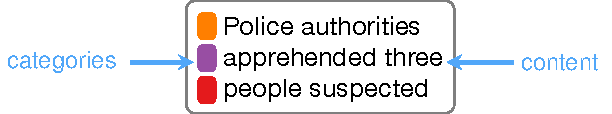
\includegraphics{event}
\caption{Visual representation of event. Text shows the content and colored badges indicate the categories.}
\label{fig:event}
\end{figure}

An event is left-aligned with its temporal value on the time axis. To reduce cluttering, an event is not visually connected to its corresponding point on the axis. Instead, it only appears when the event is hovered. The time axis is shown as a horizontal line at the bottom of all events. It includes two hierarchical temporal scales, changed dynamically according to the range of the visible events. For example, the time axis in \autoref{fig:sl-overview} shows \emph{month} and \emph{day} but they can be switched to \emph{year} and \emph{month} if needed to cover the range of events. This design satisfies the Technical Requirement 1 -- event representation.

\subsection{Schema}
\label{sub:schema}
As discussed in the Literature Review chapter, \autoref{sub:lr-gestalt}, Gestalt principles of grouping are commonly used to show relationships between events, most effectively \emph{connectedness} and \emph{proximity}. Therefore, we also apply these two principles in our design: events belonging to the same schema are located close together, and the background of an entire schema is colored to visually connected all of its events. Spatial grouping needs to be achieved through vertical positioning because the horizontal position of each event is already determined by its temporal information. Locating all events within a schema close together also makes it convenient to follow them chronologically (Technical Requirement 2 -- schema layout).

Munroe's hand-drawn movie narrative charts~\cite{Munroe2009} show the dynamic interactions of characters throughout the movie. Each character is represented as a curved line along a horizontal time axis; and vertical grouping of lines indicates which characters are together at a given interval. Inspired by this technique, we consider a ``schema'' as a ``character line'', connecting all of its events. However, instead of a thin line, we use a thicker path to provide enough space for displaying the content of events and to allow convenient interaction with individual events. For aesthetics, the path is connected rectilinearly, including only horizontal and vertical segments. Also,  all events are constrained by the same height to make the width of the path consistent. \autoref{fig:schema} shows two examples of schema. 

\begin{figure}[!htb]
	\centering
	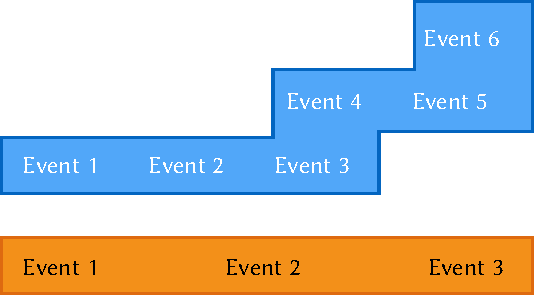
\includegraphics{schema}
	\caption{Visual representation of schema as a colored stripe. Bottom: a simple rectangle connects events that can display in the same row. Top: a rectilinear path connects events that need to locate in different rows.}
	\label{fig:schema}
\end{figure}

Putting it all together, \autoref{fig:sl-overview} shows an example of a complete SchemaLine visualization. The algorithm to produce this is described in \autoref{sec:sl-algorithm}.

\begin{figure}[!htb]
	\centering
	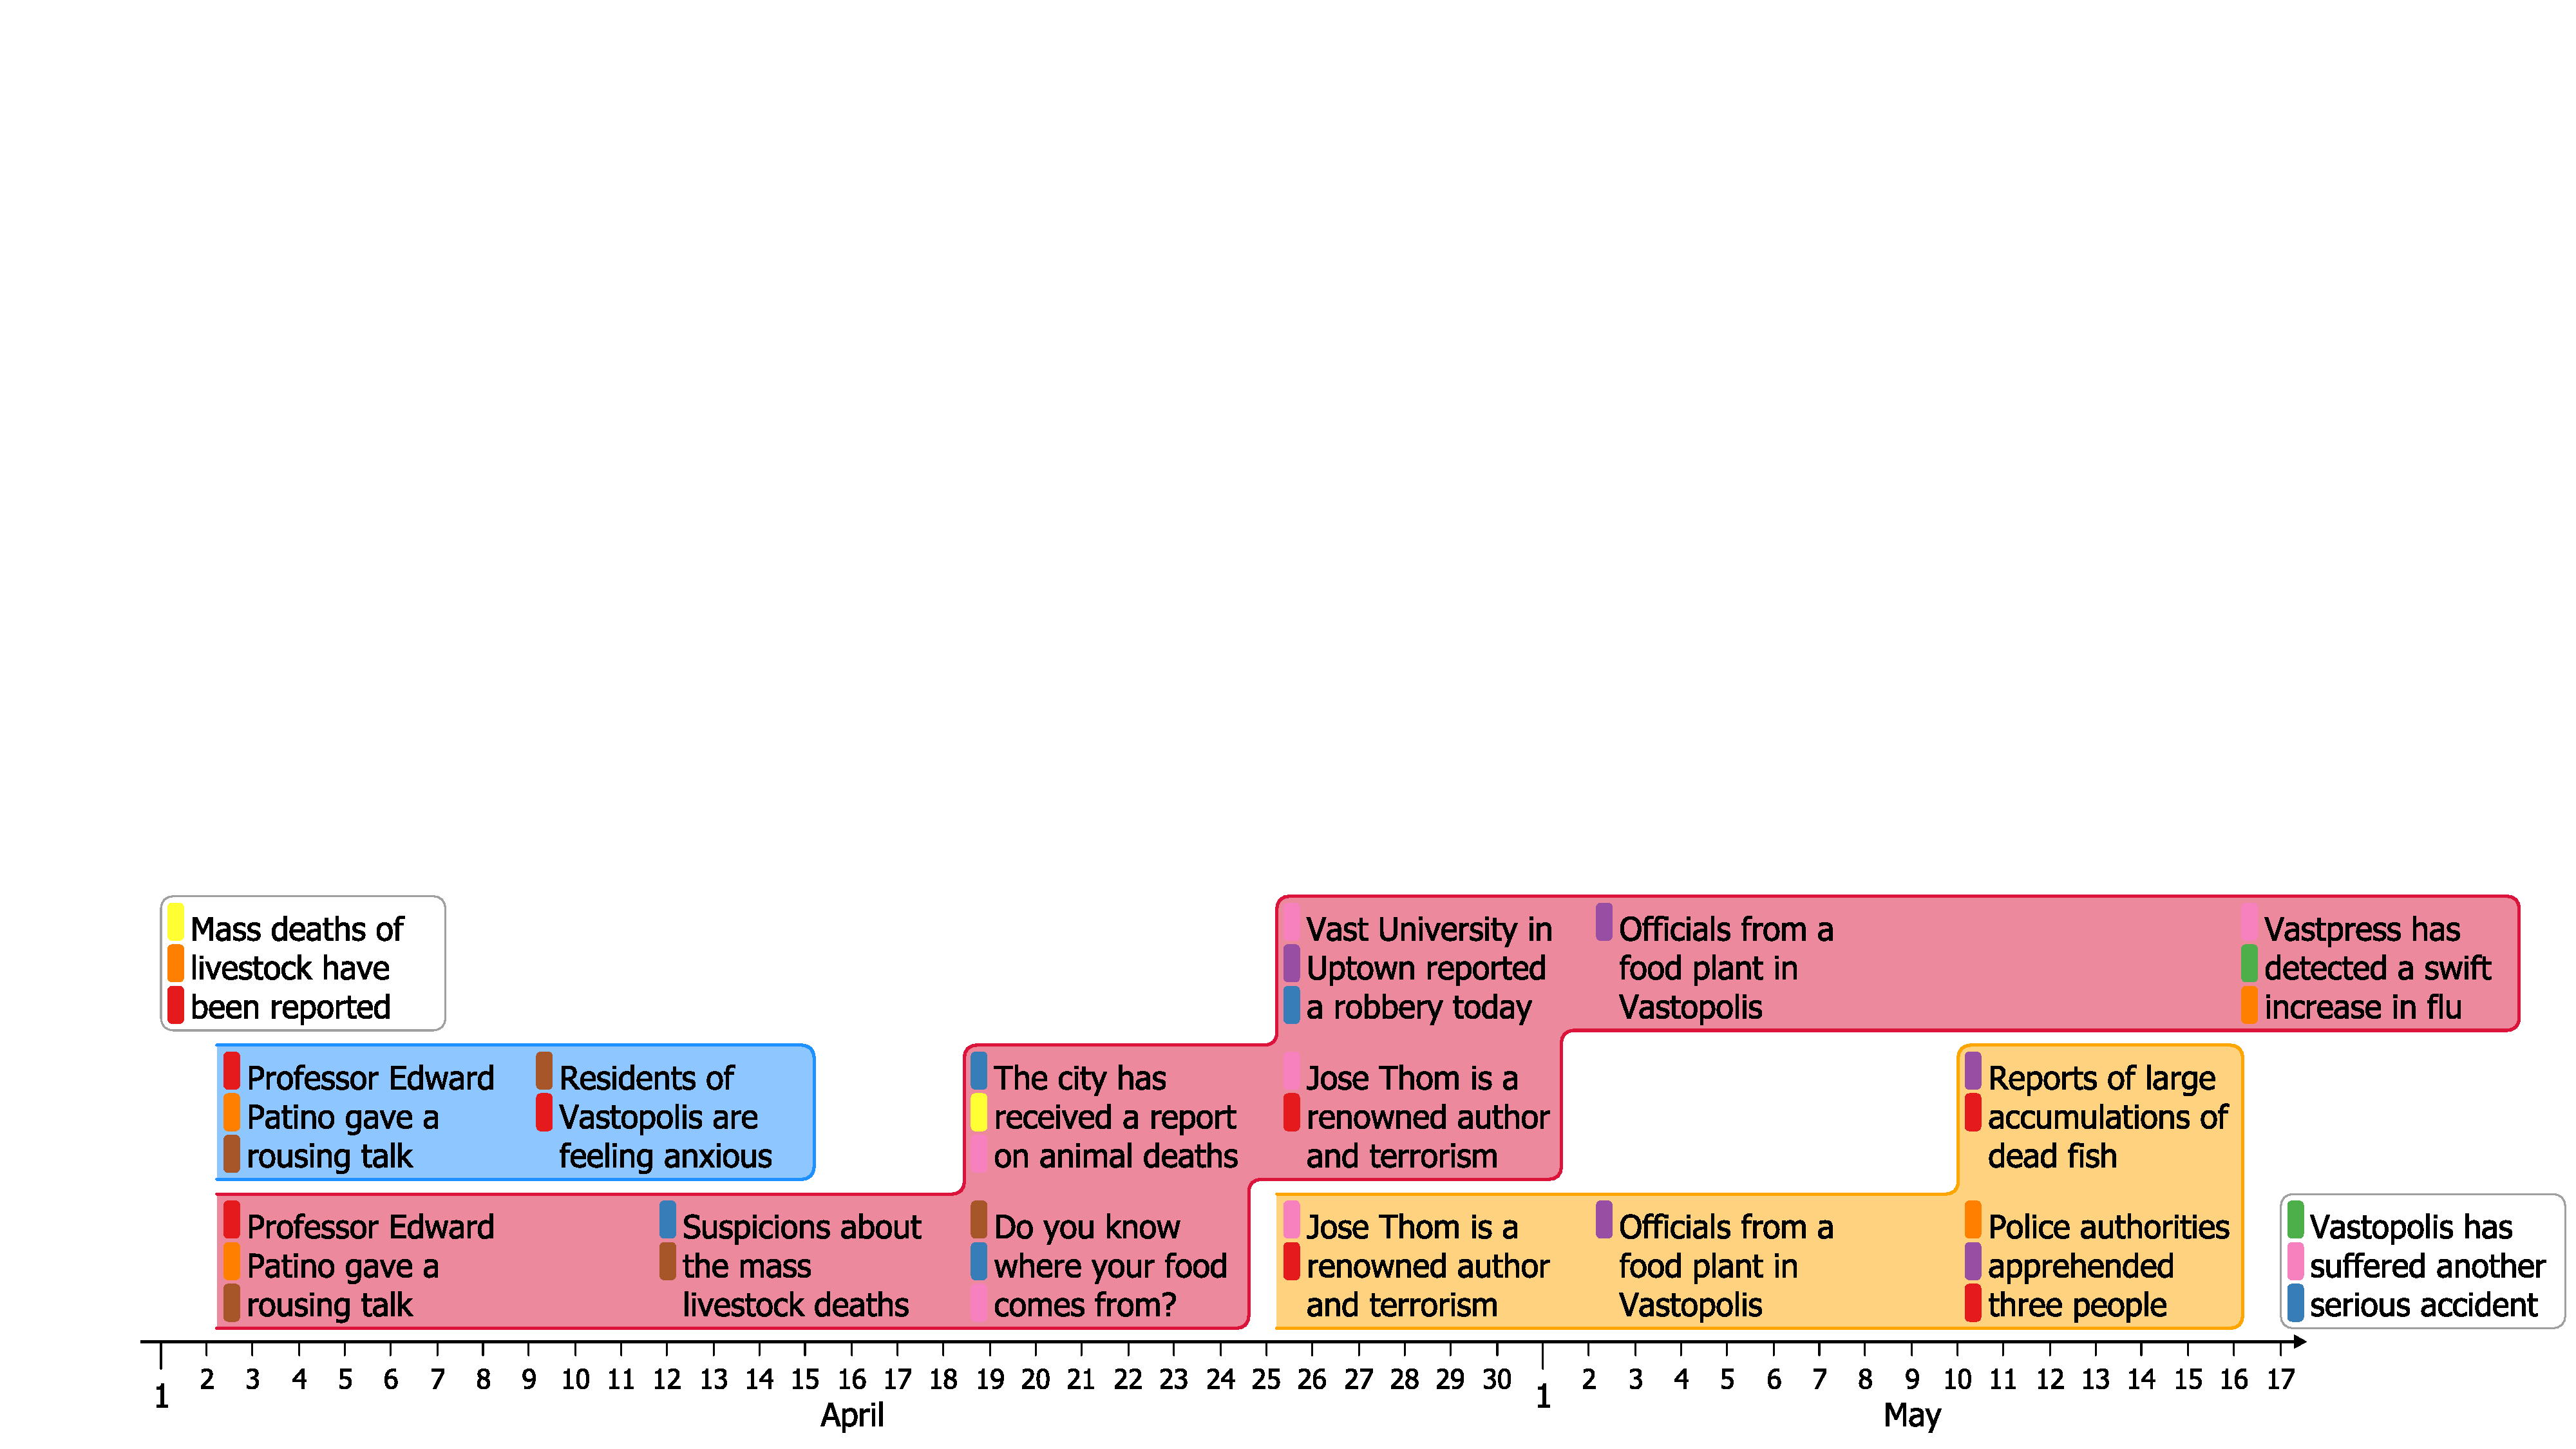
\includegraphics[width=\linewidth]{overview}
	\caption{SchemaLine visualization of annotations. Related ones are connected to form schemas.}
	\label{fig:sl-overview}
\end{figure}

\subsection{Interaction}
To enable analysts to intuitively perform sensemaking activities described in the Data--Frame model (Technical Requirement 3), we follow the design guidelines of fluid interaction proposed by Elmqvist~et~al.~\cite{Elmqvist2011}. More specifically, interactions in SchemaLine 
\begin{itemize}
	\item Produce smooth animated transitions between the state before and the state after an interaction, helping analysts to maintain their mental maps.
	\item Provide immediate visual feedback, enabling analysts to know what is happening and/or what will happen next.
	\item Manipulate directly on the visual representations of events and frames, instead of using extra menus and buttons.
\end{itemize}

During sensemaking, when the analyst recognizes a relationship of events, he or she can group them together and find an account for them (\textbf{connect data and a frame}). This activity is performed by dragging one event and dropping it onto another event, resulting a new frame consisting of these two. While dragging over, a \emph{plus} icon and a rectangle with dashed border surrounding the two events are displayed to indicate that a new frame will be created. 

The analyst can also \textbf{elaborate the frame} by adding more relevant events. This is simply executed by dropping events onto the colored stripe representing the frame. Conversely, to \textbf{preserve the frame}, the analyst can drag its events and drop them onto void space to remove them from the frame. Appropriate informative feedback is displayed in both cases: a \emph{plus} icon for elaboration and a \emph{minus} icon for preservation. \autoref{fig:add-event-frame} shows an example for elaborating the frame.

\begin{figure}[!htb]
	\centering
	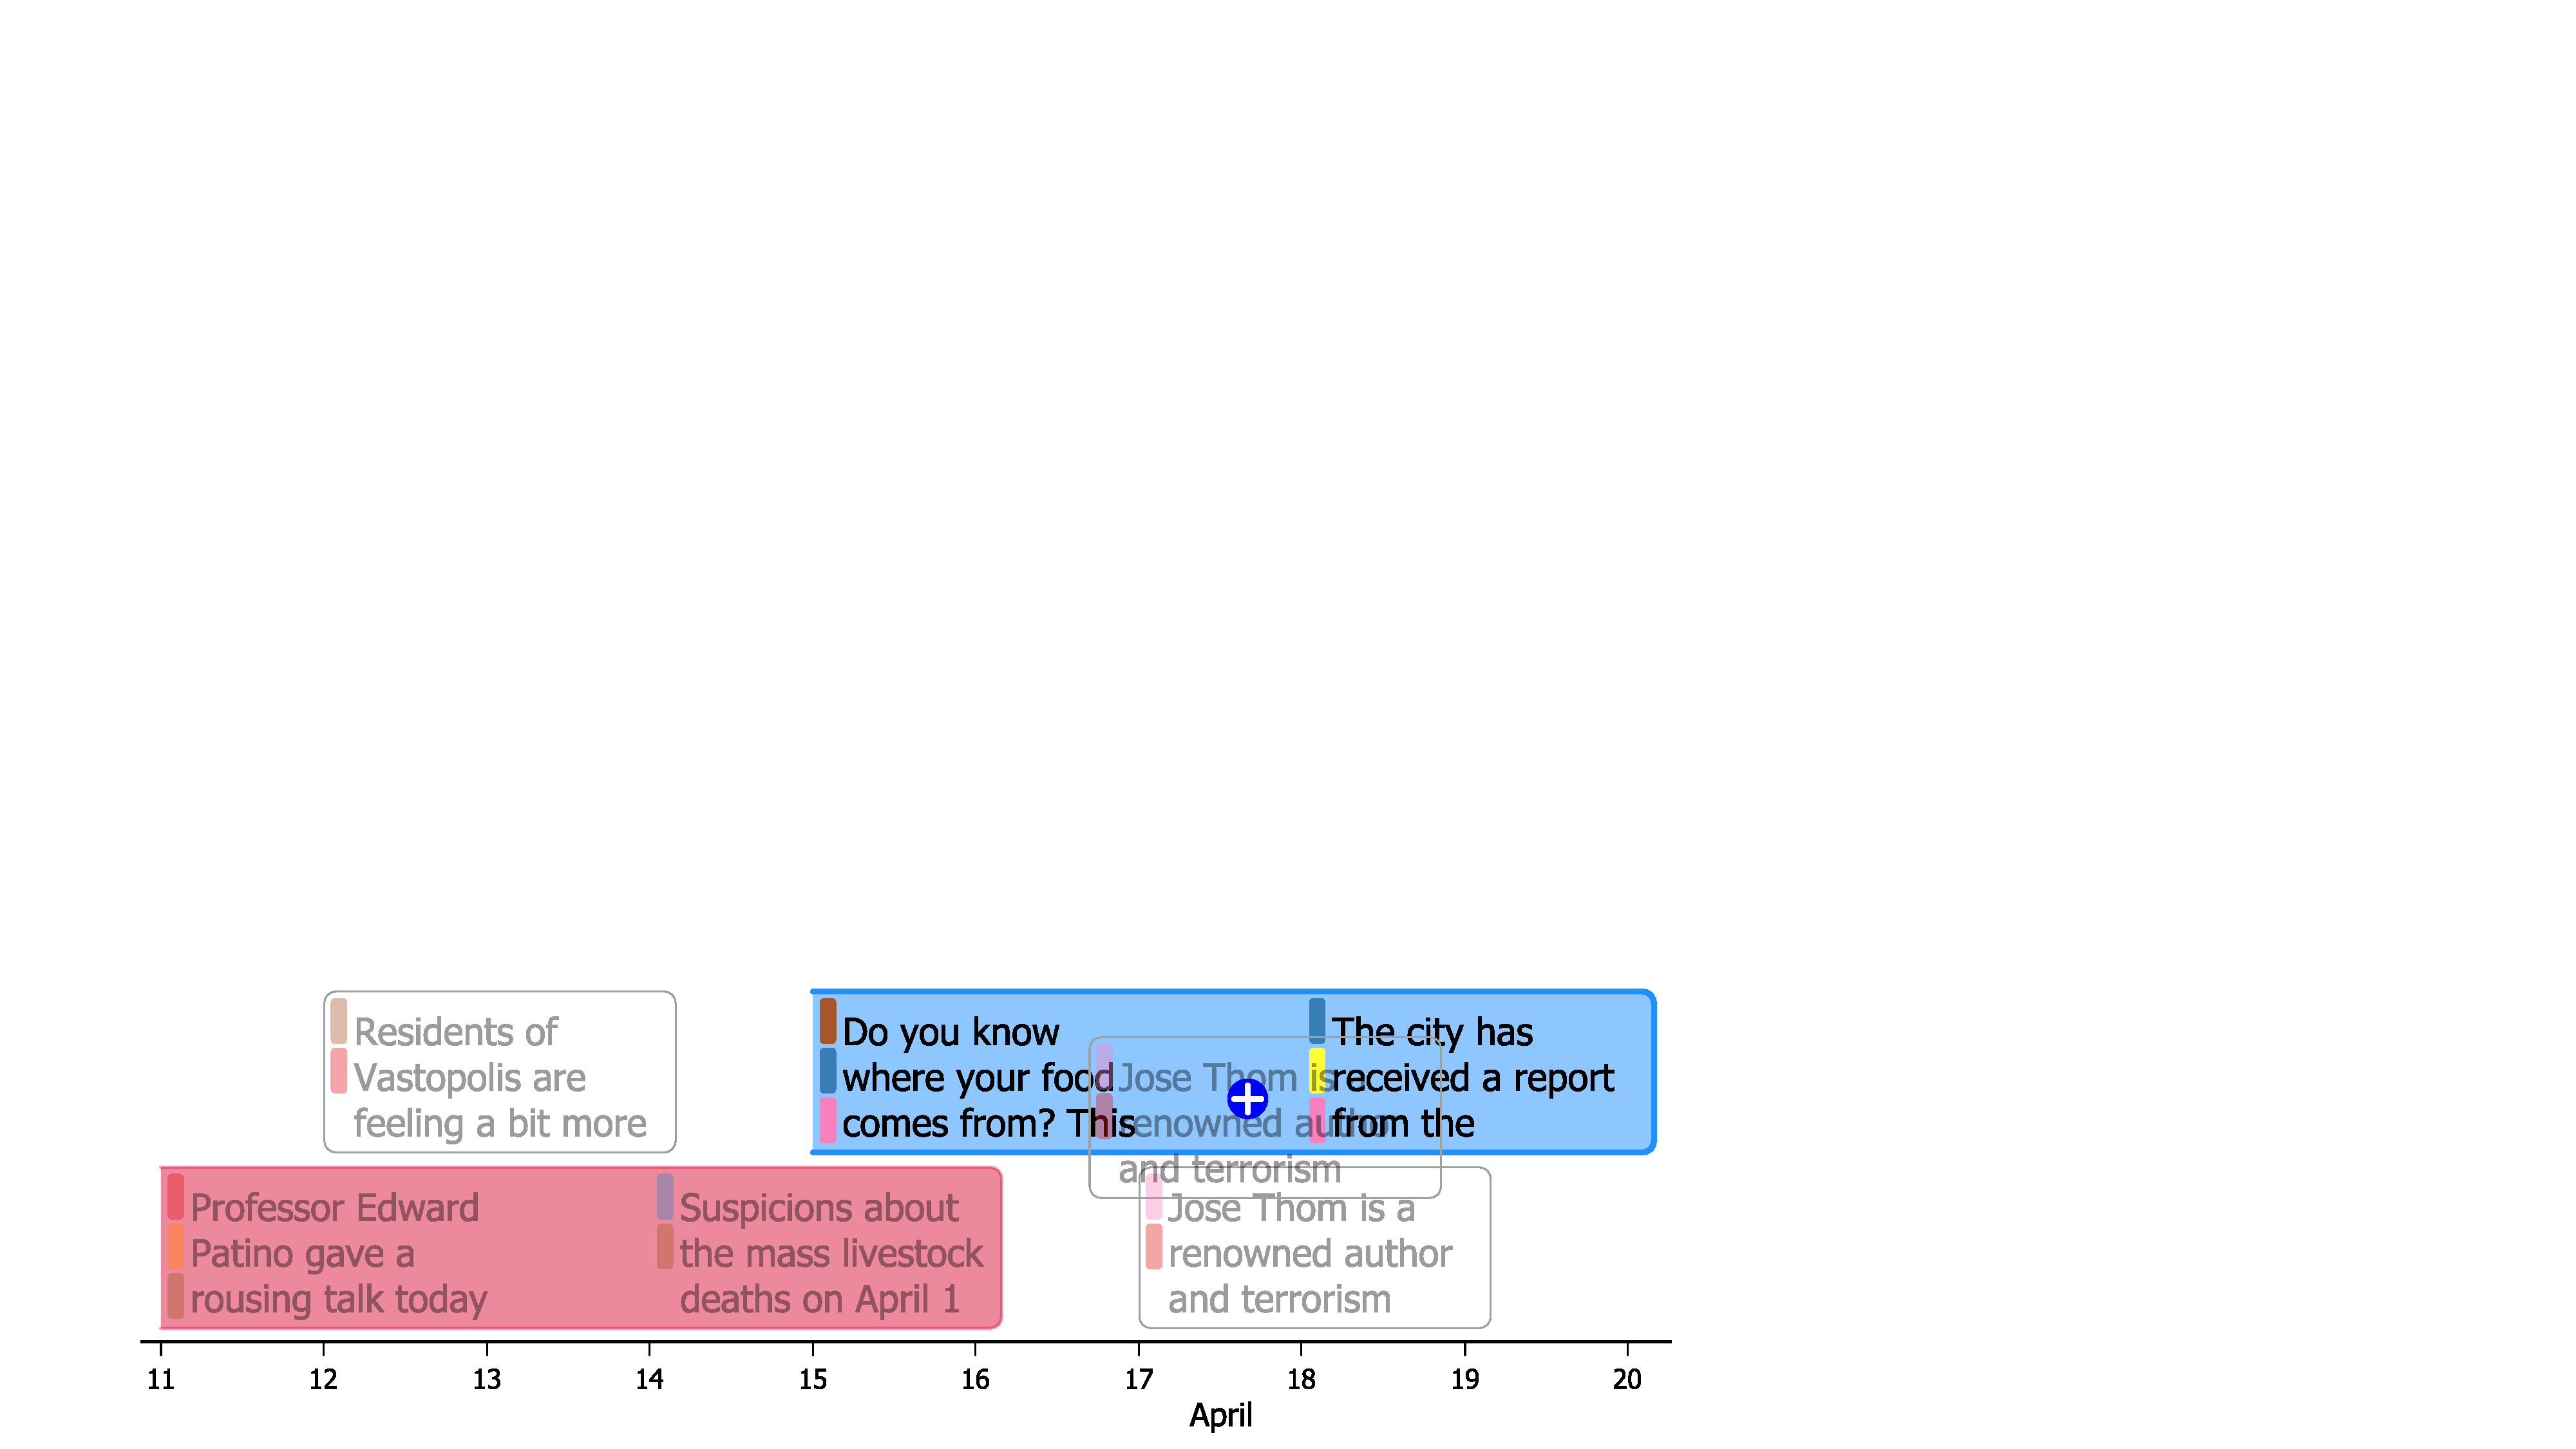
\includegraphics{add-event-frame}
	\caption{Elaborating the frame. Dragging and dropping an event onto the blue stripe to add it to that frame. The plus icon indicates the addition behavior if dropping the event.}
	\label{fig:add-event-frame}
\end{figure}

\textbf{Questioning the frame} occurs when the analyst encounters inconsistencies in data. The temporal distribution of events in the frame may suggest some concerns about the plausibility and completeness of the frame. For example, if a frame about one person contains many events in January and March, but none in February; it may be inferred that some data might be missed. To highlight a suspected event, the analyst can double-click on it with the right mouse button. The text of that event will be rendered in red to indicate that it needs more investigation. 

Depending on experience, the analyst can think of multiple explanations for the same set of data. To support \textbf{comparing multiple frames}, we enable the analyst to duplicate events and construct similar frames. By default, dragging an event from one frame and dropping it onto another frame will move it to the new frame. However, holding the \emph{Control} key while dropping an event will instead copy it to the new frame. Also, when two frames are selected, they will be moved vertically next together to facilitate comparison.

The analyst can remove an event from the timeline by dropping it at the bottom of the time axis. A red \emph{remove} icon is displayed as a visual feedback. While searching for a replacement to account for inconsistent and contrary data (\textbf{reframing}), it could be useful to consider discarded data. To enable that, SchemaLine can redisplay events that were removed earlier with half transparency to distinguish them from existing events.

When the analyst thinks that the existing frame cannot account for its data, he or she may  completely discard it and \textbf{seek a new frame}. The frame can be removed by dropping it onto void space. However, its events still remain in the timeline, enabling the analyst to exploit them. Another interaction could be useful is to combine two sets of events together -- we call it ``merge frames''. This can be performed by dragging one schema and dropping it on top of the other schema.
\section{Visual Design}
\label{sec:interface}

\subsection{Event}
An event is represented by a rounded rectangle with a short text inside summarizing its content. All rectangles have the same height to provide a consistent appearance, especially when they are later connected to form a schema (Section \ref{sub:schema-outline}). Rectangles are assigned the same maximum width and long texts are trimmed to fit into their rectangles. The full content of an event will be displayed when it is hovered. Events can include categorical attributes. For example, in news reports, the themes of an article can be sport, fashion or both. Inside the border of an event, small colored rectangles are added to the left of its text to indicate its categories. Only around 12 colors can be distinguished simultaneously in the human view~\cite{Munzner2014}. We choose Set 1 of qualitative colors from ColorBrewer~\cite{Harrower2003} for the colormap. The eight most appeared categories are displayed using these colors and other categories share the same different color. We also plan to combine color with another channel such as texture to increase the number of differentiated categories in the future work. Figure~\ref{fig:event} shows an example of event with three color-coded categories.

\begin{figure}[ht]
\centering
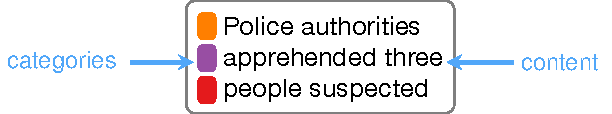
\includegraphics[width=.5\columnwidth]{event}
\caption{An event with three categories. The event is represented as a rounded rectangle with a summarized text inside. On the left side of the text, small color-coded rectangles indicate its categories. The event is positioned along the time axis at when it happens -- 8th of May.}
\label{fig:event}
\end{figure}

An event is left-aligned with its temporal value on the time axis. To reduce cluttering, an event is not visually connected to its corresponding point on the axis. Instead, when the mouse hovers an event, its time point on the time axis is highlighted. The time axis is shown as a horizontal line at the bottom of all events. It consists of two hierarchical temporal scales, which are changed dynamically according to the range of the displayed events. For example, Figure~\ref{fig:event} shows two scales: ``month/day'', but they can switch to ``year/month'' if the range is larger.

\subsection{Schema}
\todo{do the requirements, the design choices should be justified using them}
\todo{don't define schema here. this is all about representation.}
After discovering a number of relevant events or pieces of evidence, the analyst starts combining them to form a \textit{schema}. A schema is a set of related events that are connected to each other in a certain way. For example, a schema might contain all events about a particular person. Figure~\ref{fig:schema} shows examples of schema. 

\begin{figure}[ht]
	\centering
	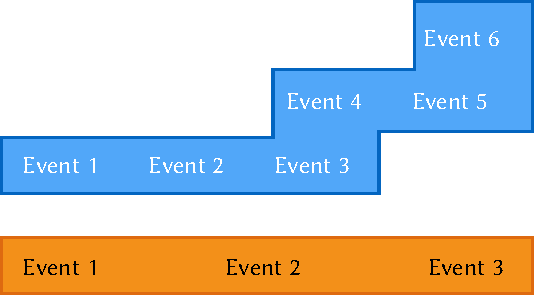
\includegraphics[width=.6\columnwidth]{schema}
	\caption{.}
	\label{fig:schema}
\end{figure}

\begin{figure}[ht]
\centering
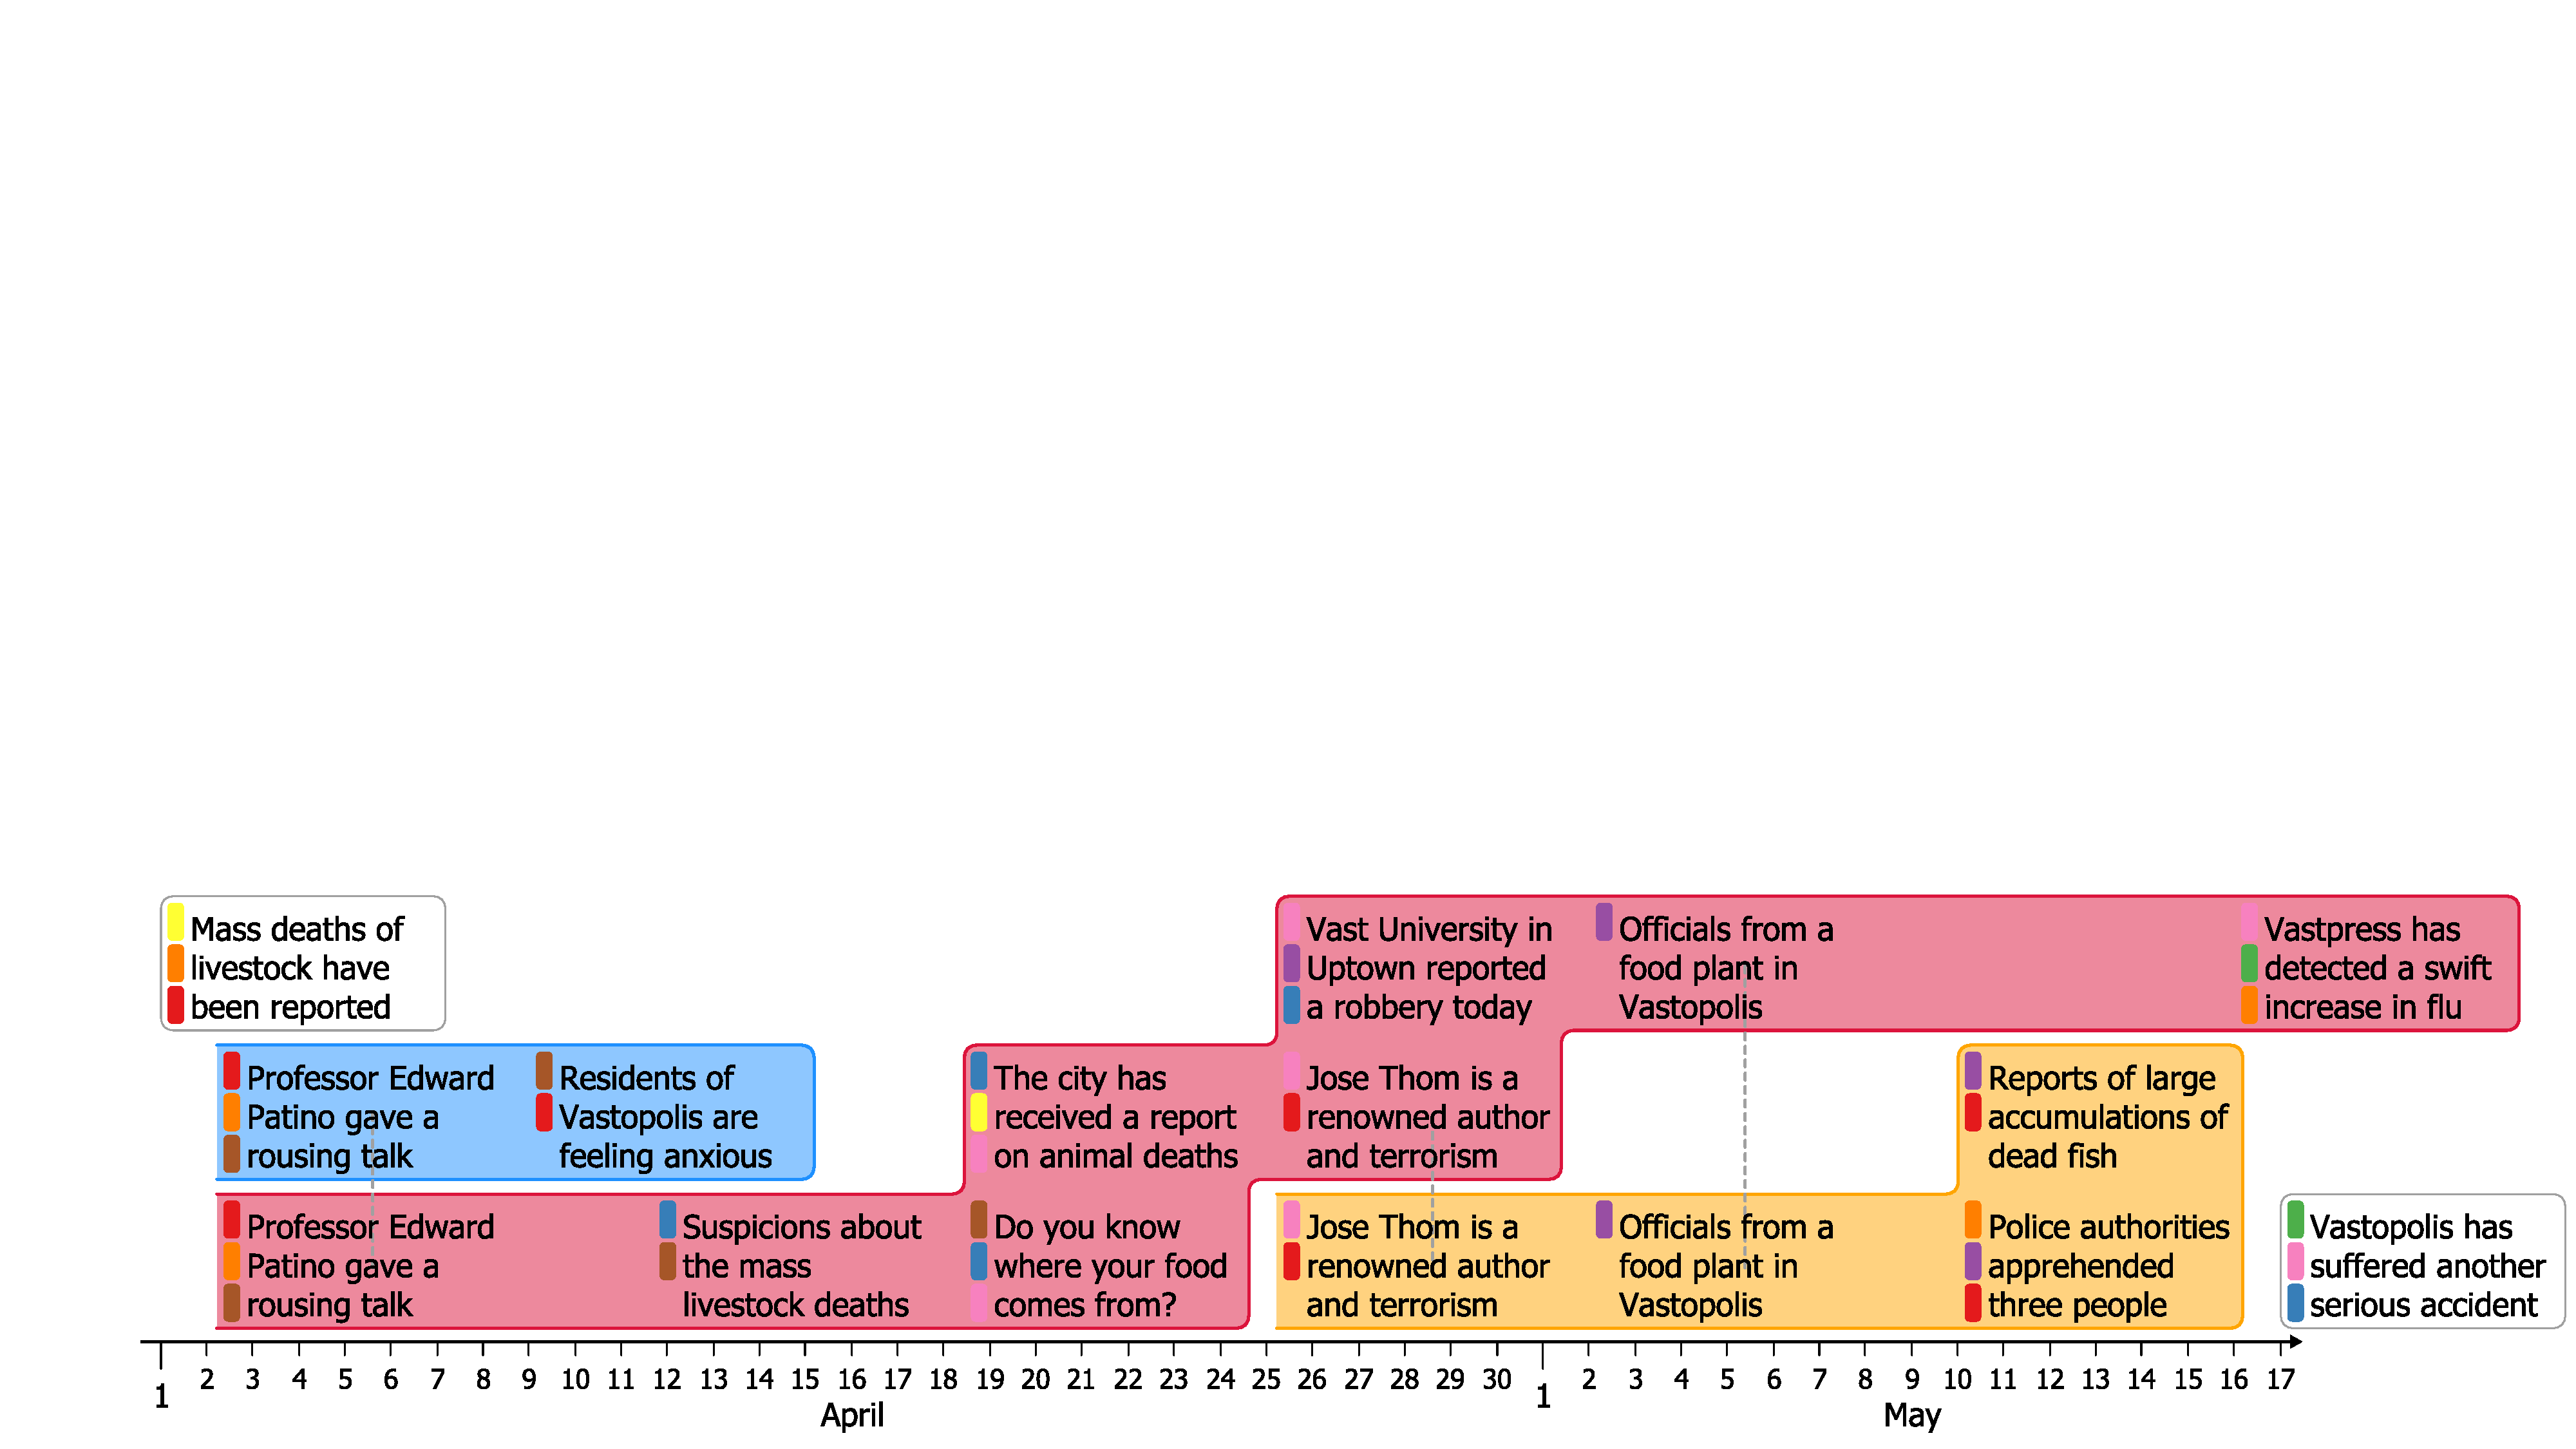
\includegraphics[width=\linewidth]{teaser}
\caption{SchemaLine: each piece of text is an analyst note, positioned along the time axis at when the event happened. Related notes are linked together to form a ``schema'' or ``frame''. There are three frames in this example represented as colored rectilinear paths. Small color-coded rectangles on the left side of notes are ``categories''.}
\label{fig:teaser}
\end{figure}

We consider several design options to connect events within a schema such as using colored/shaped icons or node-link diagrams. However, they all have some drawbacks as discussed in the Related work (Section~\ref{sec:relatedwork}). Computational methods that allow visualize a large number of events with different themes such as ThemeRiver~\cite{Havre2002} do not work either because individual events and interactions are more essential in SchemaLine. \note{I don't quite understand what the `computational' means and the argument follows} Also, it should be easy to follow events within a schema in temporal order. We decided to visualize each schema as a colored stripe, which is inspired by Munroe's hand-drawn visualization~\cite{Munroe2009}. A character line in Munroe's work connects all events happened to that character. Similarly, our schema is a color stripe connecting all events belonging to it. Instead of using a thin line, we use a path with unique width (an event's height) to make enough space to display the event's summary text and allow interaction with individual notes. A rectilinear path is employed to provide a nice visualization rather than direct connection between events. 
%\section{Layout and Outline}
\label{sec:sl-algorithm}
This section discusses how to produce the SchemaLine visualization such as the one in \autoref{fig:sl-overview}. The layout of schemas is generated before their outlines are computed based on the layout information.

\subsection{SchemaLine Layout}
Based on the technical requirements, the layout should satisfy these conditions: 
\begin{enumerate}
	\item \textbf{Horizontal position}. Along the time axis, events should be located accurately at when they happen, if possible. This is to meet Technical Requirement 1 -- event representation.
	\item \textbf{Relative order}. However, to address scalability, events can be shifted horizontally as long as their relative order is maintained: $x(e_1) < x(e_2)$ if and only if $e_1$ happens before $e_2$, where $x(e)$ is the horizontal position of event $e$.
	\item \textbf{Overlap free}. Events and schemas are not allowed to intersect each other.
\end{enumerate}

To meet these conditions, we design a layout algorithm consisting of the following four steps (\autoref{fig:sl-layout-overview}):
\begin{enumerate} 
	\item Order the schemas vertically based on their number of events.
	\item For each schema, locate its events satisfying the aforementioned requirements.
	\item Compact the schemas following the order computed in the first step.
	\item Locate the remaining events that do not belong to any schemas. 
\end{enumerate}

\begin{figure}[!htb]
\centering
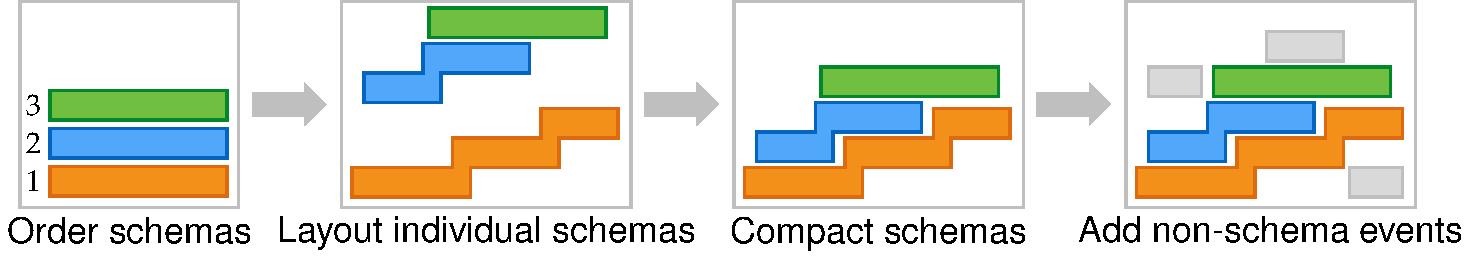
\includegraphics[width=\linewidth]{layout-overview}
\caption[Summary of SchemaLine layout algorithm]{SchemaLine layout algorithm consisting of four steps. First, the vertical order of schemas is computed. Second, the layout of each schema is generated independently. Third, the schemas are compacted based on the computed order. Last, events that do not belong to any schemas are added to the visualization.}
\label{fig:sl-layout-overview}
\end{figure}

\subsubsection{Order Schemas}
As explained in \autoref{sub:schema}, schemas are vertically stacked to apply the \emph{proximity} principle. This step computes the vertical order of all schemas based on their number of events: the schemas with more events are located under the one with less events. This ordering is based on an assumption that larger schemas (in terms of the number of events) are more relevant than smaller ones, thus are located closer to the time axis. If two schemas consist of the same number of events, the one with longer time range is located under.

\subsubsection{Layout Individual Schemas}
\label{sub:layout-schema}
The second step is to produce the layout for each schema. Events that are members of multiple schemas are replicated, allowing the layout of each schema to be generated independently. Events within a schema are sorted chronologically and added to the timeline in that order. Because all events have the same height, only the row level and horizontal position of each event are needed to computed as follows. 

Initially, an event $e_i$ is located on the same row as the previous one $e_{i-1}$ and at the position proportional to its temporal value (Condition 1 -- horizontal position). If these two events are separate, $e_i$ stays at where it is. Otherwise, two cases will be considered. First, if $e_i$ happens at the same time as $e_{i-1}$, it will be located on the upper row and at the same horizontal coordinate as $e_{i-1}$. Second, $e_{i-1}$ is tentatively shifted to the left to make space for $e_i$, as discussed next. If the shift is unsuccessful, $e_i$ will be located in the upper row as in the first case.

\paragraph*{Shifting Events}
To accommodate more events, the accuracy of the horizontal positions of events can be sacrificed. An event can be shifted horizontally to the left to make space for other events. However, an event should not be shifted too far from its accurate position to avoid misinterpretation from analysts. We set that shifting limit to the width of the event so that the event rectangle still covers its time point on the time axis and provides a reasonable indication of its accurate position. 

During shifting, it is essential to make sure that events do not overlap each other (Condition 3 -- overlap free). Considering an event $e_{i-1}$ is shifted to make space for $e_i$, if it overlaps with another event $e_{i-2}$, then $e_{i-2}$ should be shifted as well. Eventually, all events located on the way of the movement should also be shifted. It is also essential to make sure that the relative order between events is still correct after shifting (Condition 2 -- relative order). Otherwise, events with wrong order need to be shifted as well to reestablish the correct order. Note that if two events happen at the same time, they must be located at the same horizontal position. 

\autoref{fig:layout-schema-example} illustrates the layout algorithm for one simple schema.

\begin{figure}[!htb]
	\centering
	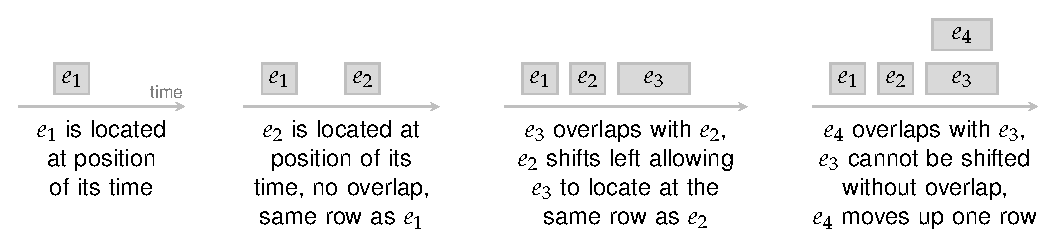
\includegraphics[width=\linewidth]{layout-example}
	\caption[Example of Schema layout algorithm]{Example of Schema layout algorithm. Four events $e_1$, $e_2$, $e_3$ and $e_4$ are added chronologically.}
	\label{fig:layout-schema-example}
\end{figure}

\subsubsection{Compact Schemas}
This third step stacks schemas in the order computed in the first step to produce an overlap-free visualization. However, to make the layout more vertically compact, it is unnecessary to strictly located schemas in that order. Schemas are processed based on the computed order, starting at the bottom row and moving upward. A schema stops when it does not overlap with previously located schemas. In the worst case, it will be located above all other schemas.

\subsubsection{Add Remaining Events}
This last step allocates events that do not belong to any schemas. Events are sorted chronologically and processed in that order. The ideal horizontal coordinate of an event is the position proportional to its temporal value; however, it can also be shifted using the \emph{shifting} method described earlier in \autoref{sub:layout-schema}. An event begins at the bottom row and moves upward until it does not overlap with any other schemas or events after possible shifts. 

\subsection{Schema Outline}
In this section, we describe a process to produce a polygonal outline covering all the event rectangles of a schema. Only horizontal and vertical line segments are used to keep the outline simple yet aesthetic as in \autoref{fig:schema}. The \emph{polygonal path} $P_n$ of a schema that contains $n$ event rectangles $R_1, R_2, ..., R_n$, ordered from left to right, is determined as follows:
\[
P_n=
\begin{cases}
R_1, & n=1 \\
P_{n-1} \oplus R_n, & n > 1
\end{cases},
\]
where $\oplus$ is an operator that appends a rectangle to a polygonal path. As described in the layout of individual schema (Section \ref{sub:layout-schema}), when a new event is added to an existing schema, it has the same row as the previous event (\autoref{fig:outline-right}) or one row higher (\autoref{fig:outline-up}). To produce an aesthetically pleasing path, two other special cases are also considered as described in \autoref{fig:outline-up-one} and \autoref{fig:outline-up-two}. Technically, a path is represented by a list of vertices and is updated when new events are added. \autoref{fig:sl-outline} illustrates how these vertices are updated, added or unchanged for all four those cases.

\begin{figure}[!htb]
	\centering
	
\includegraphics{outline-legend}\bigskip\\
	\subcaptionbox{\label{fig:outline-right}$R_3$ is on the right side of the path.}{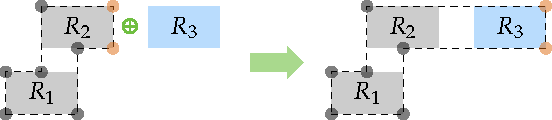
\includegraphics{outline-right}}
	
	\vspace{.5\baselineskip}
	
	\subcaptionbox{\label{fig:outline-up}$R_3$ is on top of the path.}[.43\linewidth]{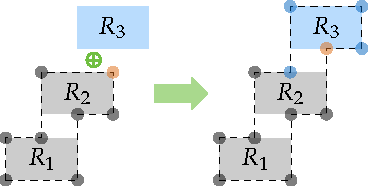
\includegraphics{outline-up}}
	\hfill
	\subcaptionbox{\label{fig:outline-up-one}Left of $R_3$ is a bit greater than left of $R_2$.}[.26\linewidth]{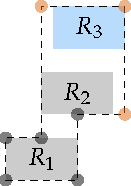
\includegraphics{outline-up-smoothing}}
	\hfill
	\subcaptionbox{\label{fig:outline-up-two}Right of $R_3$ is shorter than right of $R_2$.}[.26\linewidth]{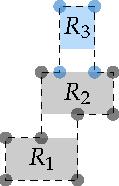
\includegraphics{outline-up-shorter}}
	\caption[Rectangle appended into a polygonal path]{Four cases when a new rectangle \colorbox{f2!40}{$R_3$} is appended \textcolor{ForestGreen}{$\pmb{\oplus}$} to a polygonal path -- representing by a dashed polygon. Vertices of the path are colored coded to describe how they are maintained.}
	\label{fig:sl-outline}
\end{figure}

After producing a rectilinear path, all corner bends are made rounded as in \autoref{fig:sl-overview}. The path is filled with the same stroke color but less transparency to make the border stand out with a darker hue. The beginning of the path does not have the border to indicate the flow of events within the path. 
\section{Sensemaking with SchemaLine}
\label{sec:interaction}

%We first discuss about the visual encoding of events and schemata; and then how sense making activities in Data-Frame model are supported in SchemaLine.

%\subsection{Event and Schema Representation}
%\label{sub:visual-encoding}
%\paragraph*{Event Representation}
%%Appearance
%An event is represented by a rounded rectangle with its left side aligned with the event's time on the timeline. To reduce cluttering, events are not constantly connected by lines to their corresponding points on the timeline. Instead, when the mouse is over an event, its time point on the timeline is highlighted. A short text is rendered inside the rectangle to summarize the event. To address the scalability of long texts, we assign a maximum width to event rectangles and trim exceeding texts. The full content will only be displayed when the note is hovered over. All events have a uniform height to give a nice overall appearance, especially when they are connected to form a schema (Section \ref{sub:schema-outline}). Quite often, events are categorical data. For example, in news reports, an article can be classified into sport, fashion or both. SchemaLine adds a small rectangle in each event to color-code its categorization. Eight different colors are supported, which are chosen from qualitative colors -- Set 1 of ColorBrewer \cite{Harrower2003}. All other categories besides eight of the most popular ones will share the same color to address the limitation of small distinguishable colors. We plan to combine colors with other indicators such as texture to increase the number of differentiated keywords in the future work. The number of maximum categories that an event can belong to is configurable to adapt the dataset characteristics. As in Fig.~\ref{fig:notes-only}, maximum four themes of an event can be displayed.
%
%\begin{figure}[ht]
%\centering
%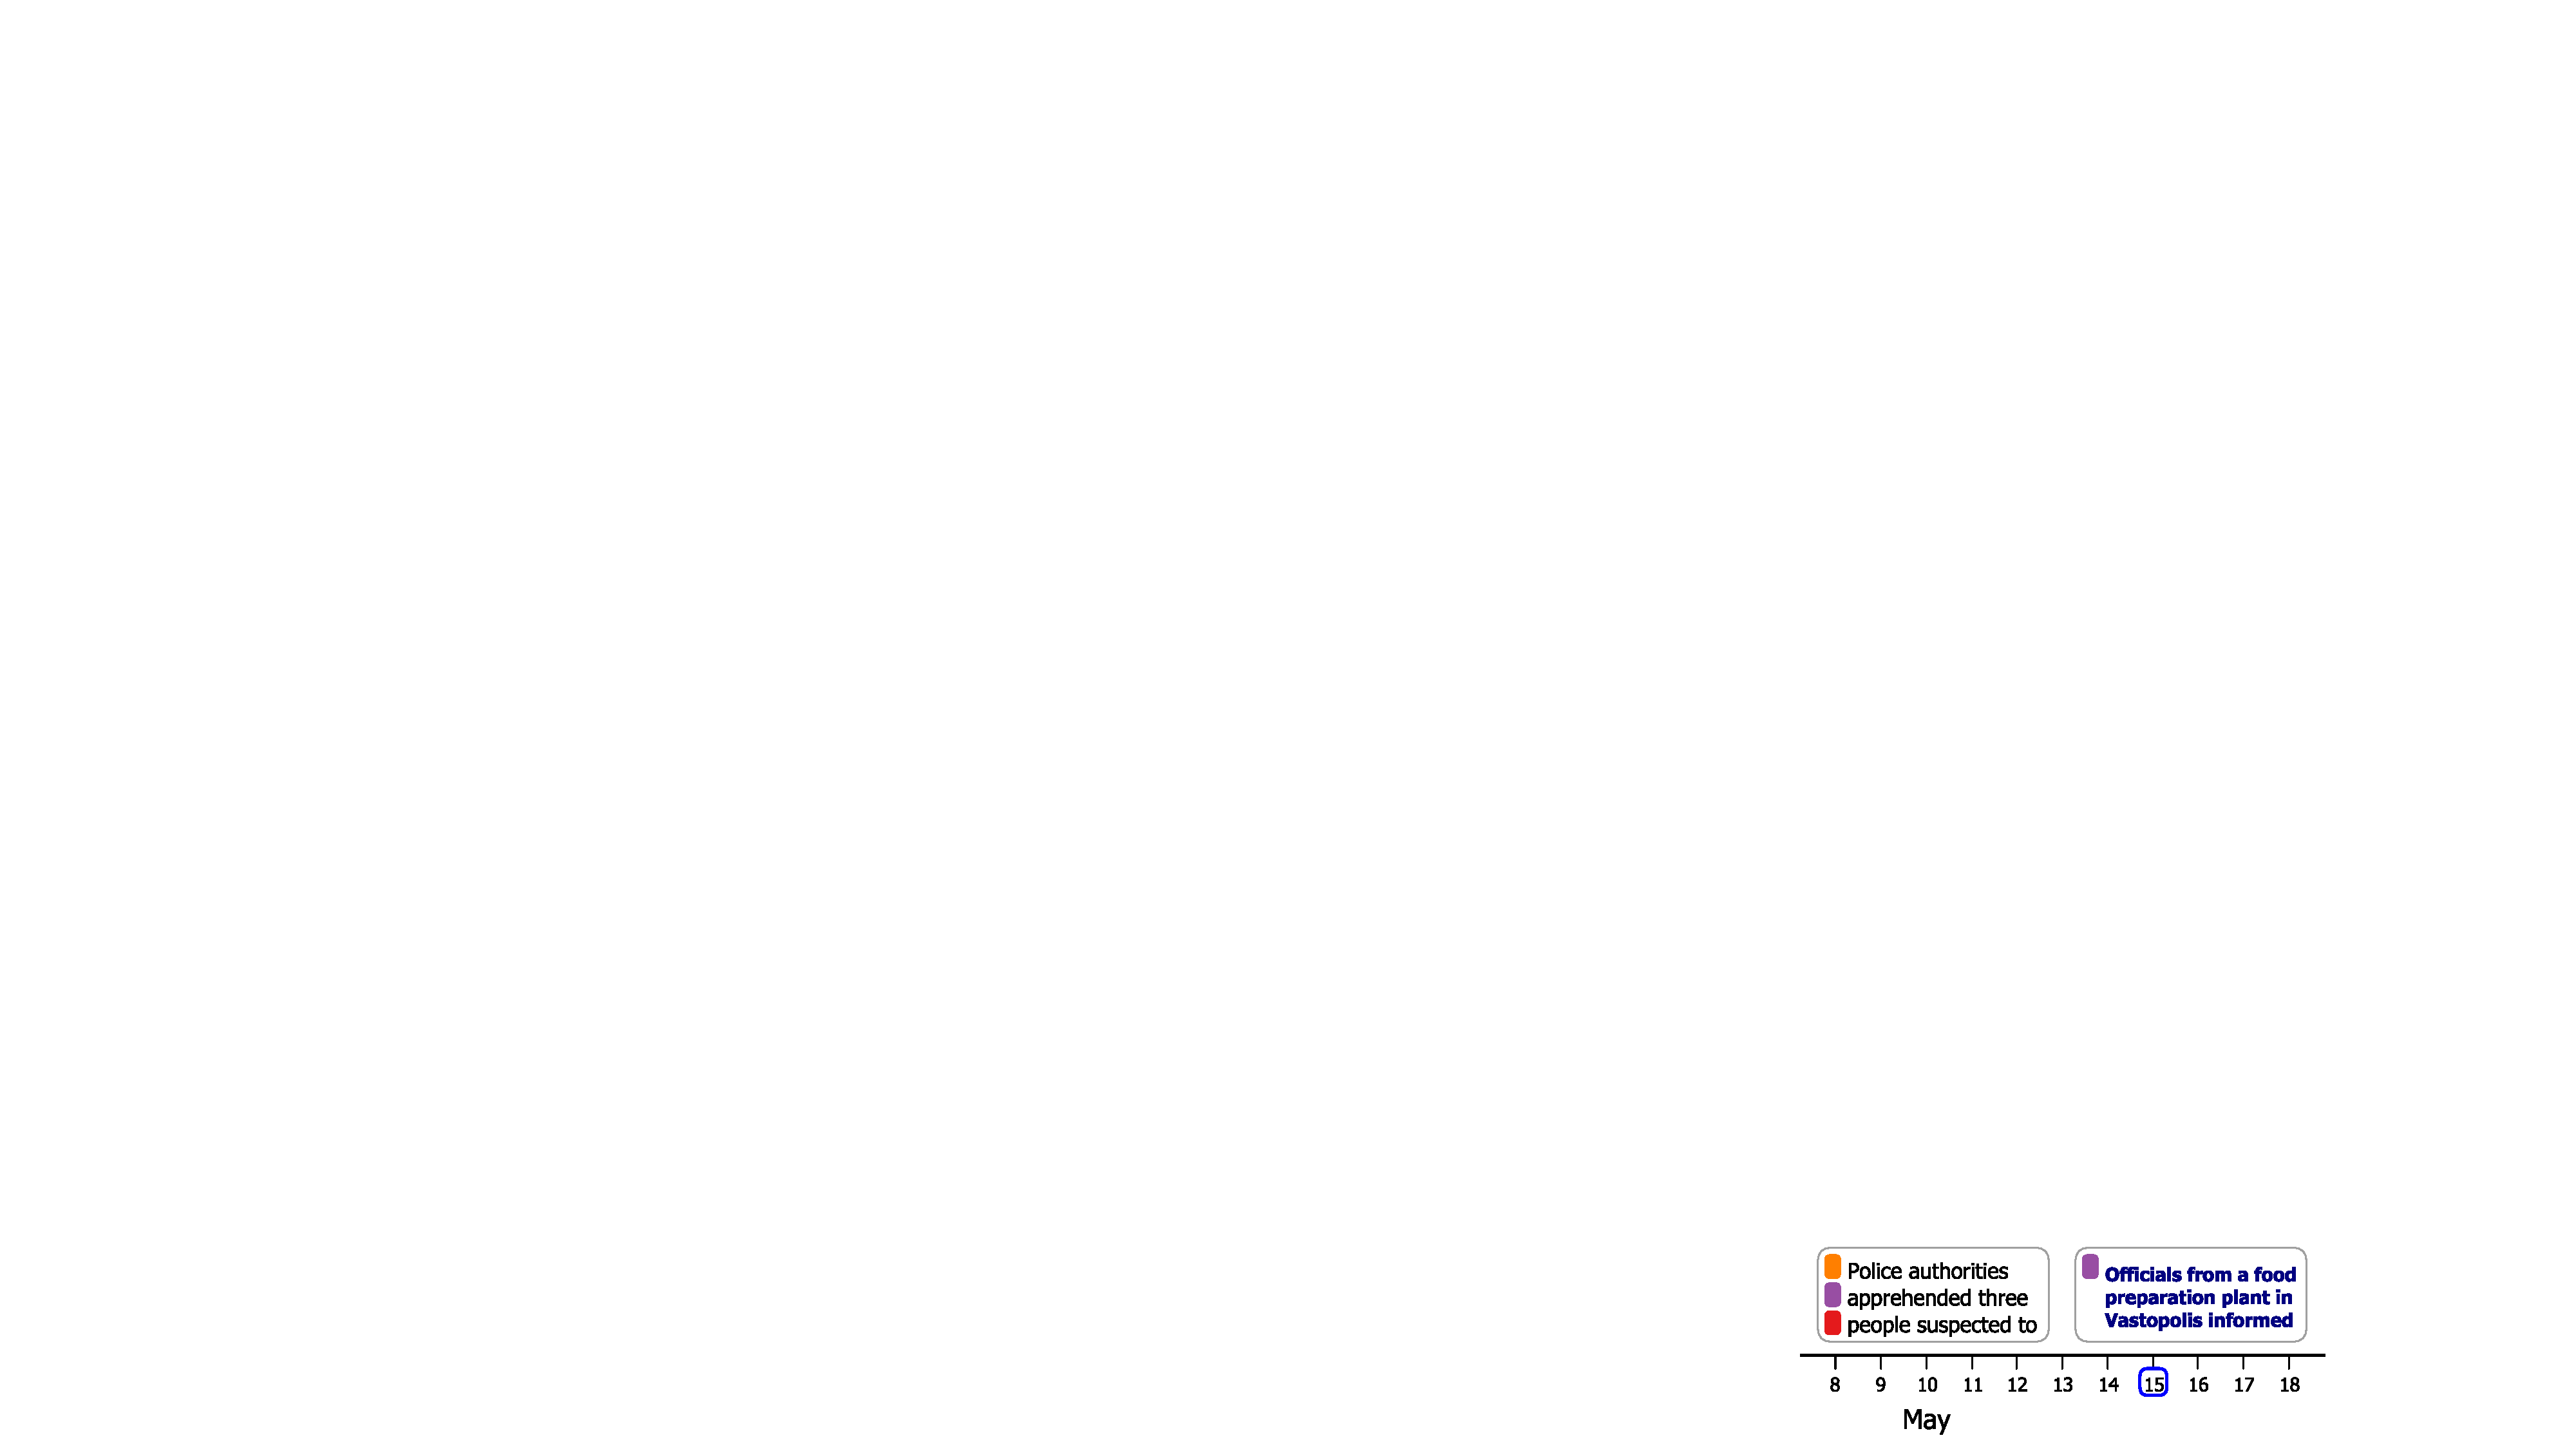
\includegraphics[width=\linewidth]{notes-only}
%\caption{Bigger texts, two events are ok, no need change time. Events are represented by rounded rectangles with uniform height and limited widths for displaying texts. On the left side of the event rectangle, there are some small color-coded rectangles to represent the event's themes.}
%\label{fig:notes-only}
%\end{figure}
%
%%Timeline appearance
%In SchemaLine, the timeline is shown as a horizontal axis at the bottom of the display. Its starting and ending points change dynamically to cover the time span of all events. The timeline consists of two temporal scales. These two scales can also be changed dynamically according to the displayed events. For example, they change from ``month/day'' to ``year/month'' to accommodate large interval increases.
%
%\paragraph*{Schema Representation}
%After discovering a number of relevant events or evidence, the analyst starts combining them to form a \textit{schema}. A schema is a set of related events that are connected to each other in a certain way. For example, a schema can contain all events about a particular person. Multiple schemata can be composed in SchemaLine as shown in Fig.~\ref{fig:teaser}. 
%
%We consider several design options to connect events within a schema such as using colors~\cite{TimeGlider2013} or node-link diagram~\cite{Jensen2003}. However, they all have some drawbacks as discussed in the Related work (Section~\ref{sec:relatedwork}). Computational methods that allow visualize a large number of events with different themes such as ThemeRiver~\cite{Havre2002} do not work either because individual events and interactions are more essential in SchemaLine. Also, it should be easy to follow events within a schema in temporal order. We decided to visualize each schema as a colored stripe, which is inspired by Munroe's hand-drawn visualization~\cite{Munroe2009}. A character line in Munroe's work connects all events happened to that character. Similarly, our schema is a color stripe connecting all events belonging to it. Instead of using a thin line, we use a path with unique width (an event's height) to make enough space for displaying the event's summary text and possible to interact with individual notes. A rectilinear path is employed to provide a nice visualization rather than direct connection between events. An example can be seen in Fig.~\ref{fig:schema} and details of the algorithm to generate the schema layout and outline will be discussed in Section~\ref{sec:layout}.
%\begin{figure}[ht]
%\centering
%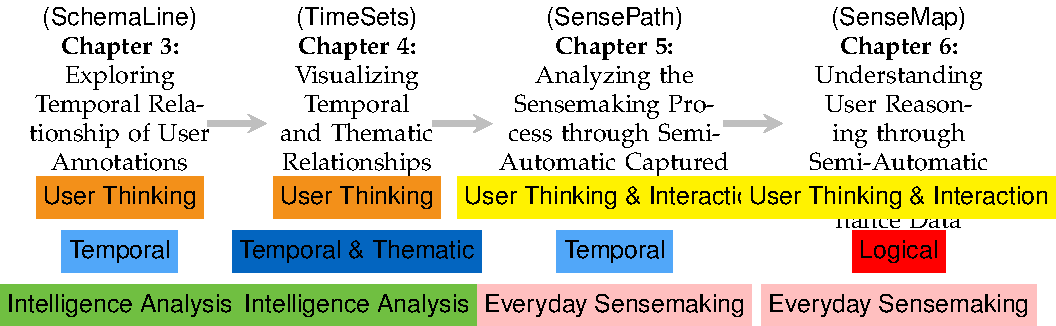
\includegraphics[width=\linewidth]{story}
%\caption{A schema with rounded corners.}
%\label{fig:schema}
%\end{figure}

%In the SchemaLine, each white rectangle is an analysis note, linking to the document in the search results that led to this discovery and positioned along the time axis at the point when the event happened. Notes can be grouped together to form a ``story''. There are three stories in this example and they are in red, blue, and orange. In the middle are the results of two searches: ``vastopolis'' and ``terrorist''. At the very top is a list of minimized searches, only showing the keywords. 


%Pirolli and Card~\cite{Pirolli2005} regarded the timeline as an effective tool for the ``Schematize'' task. A timeline can not only reveal the temporal relationships among the findings, but also have a considerable impact on how easily they can be understood. Pennington and Hastie~\cite{Pennington1991} studied the impact of evidence presentation order on juror decision making. They found that information was easier to understand when presented in chronological order and thus had a significant impact on jurors' decisions. 

%\subsection{Sensemaking with Data-Frame Model}
%\label{sub:interactive-editing}
SchemaLine is designed to support all five sensemaking activities in Data-Frame model through fluid user interactions. Following the design guidelines for fluidity proposed by Elmqvist et al.~\cite{Elmqvist2011}, SchemaLine's interactions
\begin{itemize}
	\item use smooth animated transitions between states,
	\item provide immediate visual feedback on interaction, and
	\item use direct manipulation of visual representations.
\end{itemize}

Sensemaking activities in Data-Frame model involve two different types of entities: \textit{data} and \textit{frame}. We allow direct manipulation of visual representations of data and frame, instead of invoking menus and buttons to perform actions. The first sensemaking activity in the Data-Frame model is to \textbf{construct a new frame} by connecting relevant data. It can be performed in SchemaLine by \textit{dragging one event and dropping it onto another event}. A \textit{plus} icon and a \textit{dashed rectangle} surrounding the two events are displayed to indicate that a new frame will be created. When dropping the event, a color stripe representing a frame will be formed by connecting these two events, and a smooth animated transition is used to improve user perception.

Besides dropping an event on top of another event, the user can drop it onto the color stripe to add that event to an existing frame (\textbf{elaborate a frame}). Conversely, the user can drag an event belonging to a frame and drop it onto the void space to remove it from the frame (\textbf{preserving a frame}). Appropriate informative feedback is displayed, \textit{plus} icon for addition and \textit{minus} icon for subtraction, and a smooth animated transition is used to improve user perception. Fig.~\ref{fig:drag-drop-note} shows an example of adding an event into a frame.
\begin{figure}[ht]
\centering
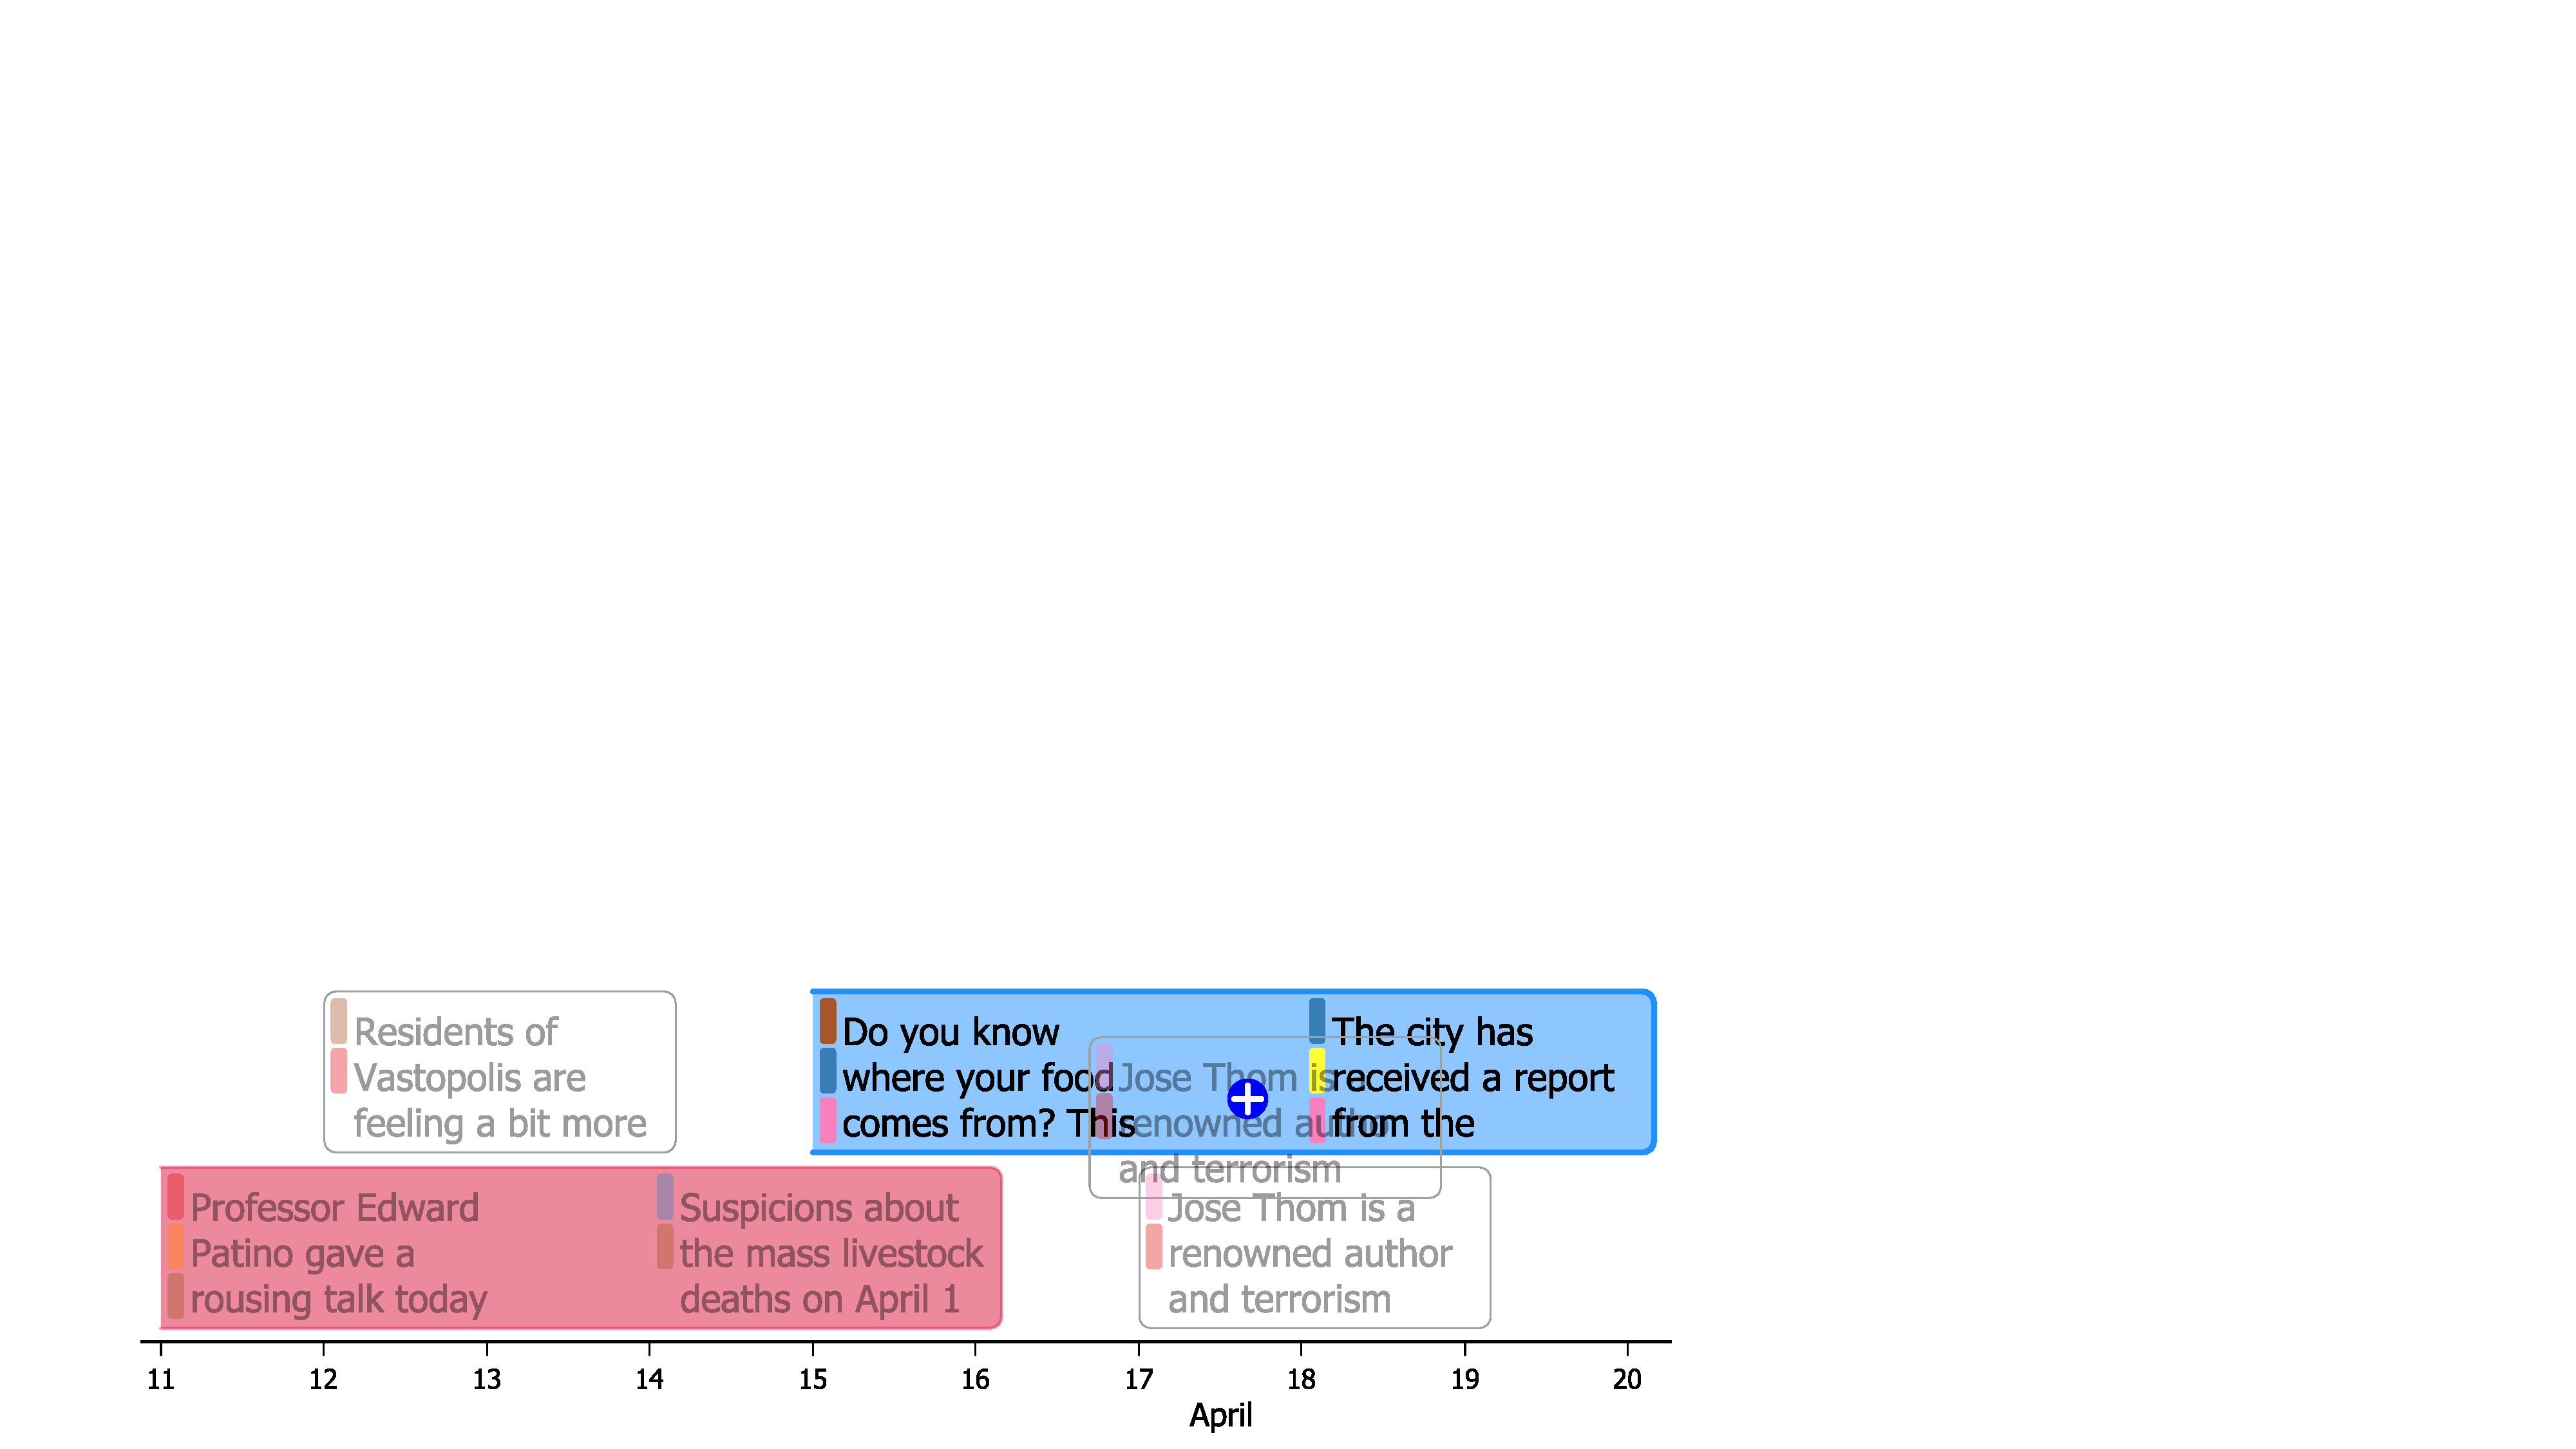
\includegraphics[width=\linewidth]{add-event-frame}
\caption{Each frame is represented as a colored stripe. Dropping an event onto the blue stripe means adding that event into the blue frame to elaborate it.}
\label{fig:drag-drop-note}
\end{figure}

\textbf{Questioning a frame} occurs when the user encounters inconsistencies in data within a frame. The temporal distribution of events in the frame may suggest some concerns about the validity or completeness of the frame. For example, if a frame about one person contains many events in January and March, but no events are found in February, then it may be inferred that there could be some data missing. The analyst can mark a suspected event by right-mouse double-clicking on it. Red color text is used to indicate that the event needs more investigation. 

Dragging an event from one frame to another frame will remove it from the old frame and add it to the new frame. However, holding \textit{Control} key when dropping will instead copy the event to the new frame. This interaction allows the analyst to duplicate events to create several similar frames and compare them (\textbf{comparing frames}). When two frames are selected, they will be moved closer together to allow easy comparison, irrespective of the frames ordering generated by the layout algorithm. The user can drag an entire frame and drop it onto another frame to merge all events together. The user can also drop the frame onto the void space to take apart the frame and release its events. This interaction is useful when the user thinks that the frame is completely wrong and wants to construct a new frame (\textbf{reframing}).

Other interactions with events are also designed to be intuitive. Left-mouse double-clicking on an event opens its full content. Dragging an event with the right mouse button can change the event's date. This feature is useful because the report date is not always the date when the event actually occurred; for example, ``yesterday there was a bomb attack in ABC''. Dragging an event outside the boundary of the timeline will remove it from the system (with \textit{remove} icon as informative feedback).

Once any change is made on SchemaLine, such as moving an event from one frame to another, an animation is shown of smooth transition between the changes to help analyst update their ``mental map''. To achieve this, the layout algorithm (Section \ref{sub:schema-layout}) computes the new event rectangle locations. Then, the outline algorithm (Section \ref{sub:schema-outline}) runs at every step of the interpolation between the old and the new locations to produce intermediate polygon paths based on the updated event locations.
\section{Evaluation}
\label{sub:sl-evaluation}
SchemaLine was integrated into an existing visual analytics system to evaluate its usefulness in making sense of temporal relationship in intelligence analysis. The integration will be discussed next and followed by a sensemaking case study.

\subsection{Application}
% Overview of INVISQUE
We integrate SchemaLine into INVISQUE~\cite{Wong2011} -- a visual analytics system designed for interactive exploration of text documents. INVISQUE provides full-text search and organizes the search results into a two-dimensional canvas, with each dimension representing a configurable attribute. For example, it may be useful to order academic articles horizontally by publication date and vertically by citation count. Search results are shown as a cluster of \emph{index-cards}, each representing a document with selected information such as publication title, date, keywords and authors. \autoref{fig:invisque} shows a screenshot of INVISQUE.

\begin{figure}[!htb]
	\centering
	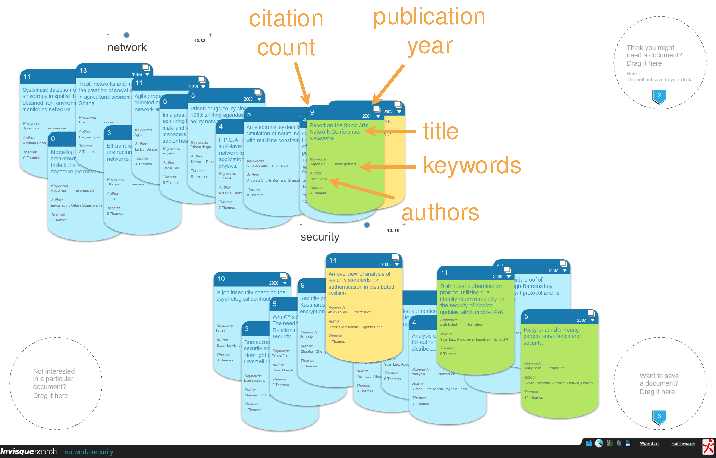
\includegraphics[width=\linewidth]{invisque}
	\caption{INVISQUE interface. It shows two clusters of search results for ``network'' and ``security'' from a publication dataset. Each index-card in a cluster represents an article with meta information displayed on it.}
	\label{fig:invisque}
\end{figure}

% Integration
We add an \emph{annotation} feature to allow analysts to record their thoughts while reading documents. Technically, the association between an annotation and its containing document should be saved for potential provenance retrieval. These annotations are important to analysts, thus are also displayed on the index-cards together with other meta information. The annotations are used  as the input \emph{events} of the SchemaLine visualization. SchemaLine is placed at the bottom of INVISQUE. After the analyst makes a note, or annotation, it is immediately added to SchemaLine as a new event. Double clicking on an event will open the document containing that note as an index-card, enabling the analyst to quickly reexamine the original information source.

% Attribute mapping
The \emph{temporal information} of documents, such as ``publication date'', is initially assigned to that of events, and can be corrected later by analysts. This feature can be useful because the report date is not necessary the same as the date when the event actually occurred. For example, a news article published today can be written about a bomb attack that happened several days ago. The analyst can make the correction by dragging an event with the right mouse button along the time axis and dropping it at the desired date. 

The \emph{label} of an event simply maps to the content of an annotation itself. In INVISQUE, we color code search keywords that contain annotated documents, and use them as \emph{categories} for events. Because a document can be returned from different searches, it can thus contain multiple categories. This mapping provides context for the annotations: what did I search for (the original keyword) and what are other related concepts (other search keywords returning the same document)? This context may help analysts discover interesting patterns through their annotations. \autoref{fig:invisque-schemaline} shows a screenshot of INVISQUE with SchemaLine integrated.

\begin{figure}[!htb]
	\centering
	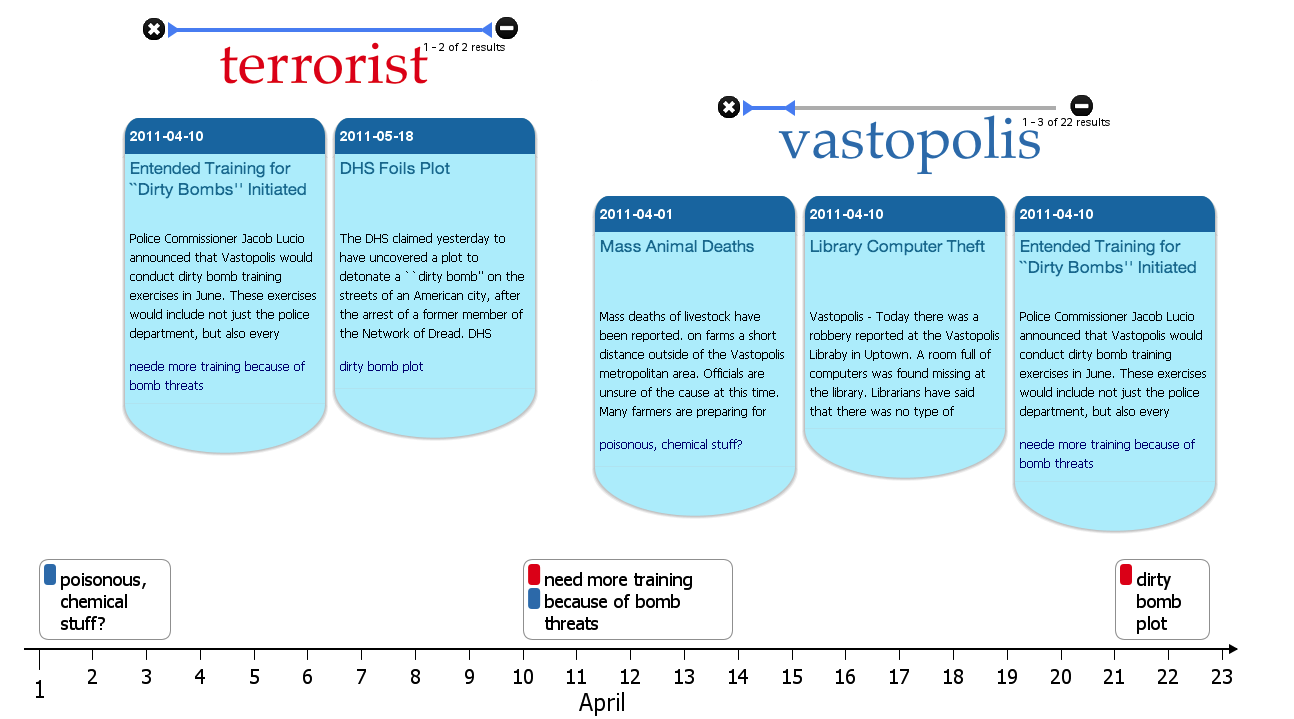
\includegraphics[width=\linewidth]{invisque-schemaline}
	\caption{INVISQUE with SchemaLine at the bottom. The timeline consists of three events, which are notes taken by an analyst. Color coded categories of events indicate keywords that were searched for.}
	\label{fig:invisque-schemaline}
\end{figure}

\subsection{Case Study}

\subsubsection{Design}

\paragraph{Method}
Evaluating the usefulness of SchemaLine in supporting sensemaking can be categorized as \emph{evaluating visual data analysis and reasoning} -- one of the seven scenarios in evaluating information visualization proposed by Lam~et~al.~\cite{Lam2012}. The goal of this evaluation scenario is to explore whether and how a visualization tool supports participants to make sense of the given tasks and generate relevant knowledge. During solving sensemaking tasks, participants may employ various strategies. Their processes and outcomes are also highly context-sensitive, making it difficult to quantify and compare their performance. Therefore, sensemaking evaluations are typically case studies with real-world tasks performed by domain experts. We conducted a case study to explore how SchemaLine supports analysts to solve an intelligence analysis task, focusing on how it enables them to perform sensemaking activities in the Data--Frame model. However, due to a limited access to these resources, we instead use a realistic investigative task with graduate students.

\paragraph{Task}
We used the task from Mini Challenge 3 of the IEEE VAST Challenge 2011~\footnote{\url{http://hcil2.cs.umd.edu/newvarepository/VAST Challenge 2011/challenges/MC3 - Investigation into Terrorist Activity/}}, which requires the participants to identify any imminent threats from the given dataset. We chose this task because it resembles a real intelligence task, demanding analysts to read many documents, extract relevant pieces of evidence and assemble them in order to derive insight and find a reasonable answer to the given question. Also, the solution was provided and well-tested by the community, making it possible to assess participants' performance. The participants were given INVISQUE with SchemaLine integrated to solve the task. 

\paragraph{Dataset}
The original dataset contains more than four thousand news reports, 36 of which are relevant to criminal activities and are manually added by the Challenge committee. Both participants in our pilot test failed to find any imminent threats after one and a half hours. Most of their time was spent on reading long (more than 500 words) but irrelevant documents. The reason could be that INVISQUE does not support text-mining features such as entity extraction, which is crucial in analyzing a large document collection. However, the goal of this evaluation was to assess how SchemaLine can provide additional sensemaking support to INVISQUE rather than assessing INVISQUE itself. Therefore, in the main study, we removed all irrelevant documents that are not part of the ground truth to make the dataset size more manageable. The new dataset only contains the 36 relevant documents, 29 of which are correct answers including five criminal activities: food poisoning (13 documents), hacking (3), dirty bomb (6), arms trafficking (4), and money laundering (3). Other documents are isolated cases, acted as false leads. We expected that participants could complete the task within a reasonable amount of time, without affecting the goal of the study. 

\paragraph{Participants and Procedure}
We were unable to recruit real intelligence analysts for the study. Instead, we recruited three graduate students with different backgrounds:  one in visual analytics (surrogate for visualization expert -- \textbf{P1}), one in law (surrogate for domain expert -- \textbf{P2}), and one in computer network (neutral background -- \textbf{P3}). After being introduced features of INVISQUE and SchemaLine, participants had a chance to practice with a trial sensemaking task for 15 minutes. The main task was followed and lasted for one hour. The participants were asked to report the criminal activities they had discovered with supporting evidence. Semi-structured interviews were followed to gain deeper understanding of the sensemaking processes.

\subsubsection{Results and Discussion}
We first summarize the three sessions and present our collective findings next.

\paragraph{Participant 1}
\textbf{P1} began searching for ``bomb'', examined the search results, and searched for  a refined keyword ``dirty bomb''. He took notes in three documents and then linked these notes together (\emph{connect data and a frame}). He then searched for ``Network of Dread'', which was mentioned in one of documents related to the dirty bomb attack. He took a note in the new returned document and dropped it onto the ``dirty bomb'' schema (\emph{elaborate the frame}). While investigating, he encountered an article about a man carrying a frozen turkey having wires coming out of it, which was suspected as a bomb. At first, he dropped the ``turkey bomb'' note onto the ``dirty bomb'' schema. Then, he wondered whether it was a real bomb. After thinking for a while, he removed it out of the schema (\emph{preserve the frame}). \textbf{P1} found the ``dirty bomb'' attack with 4/6 correct pieces of evidence. \textbf{P1} took many notes in documents related to the ``food poisoning'' case; however, he could not link them together because he said that ``I'm not familiar with bio-attack so I couldn't think of it as a threat''. 

\paragraph{Participant 2}
\textbf{P2} took an overview step before searching. He quickly looked at all 36 document titles to have a glimpse of the dataset as well as to detect potential search keywords. Then he searched for ``animal deaths'', read the results, took notes and grouped them together (\emph{connect data and a frame}). He was satisfied with the evidence he found for that crime and switched to read another interesting article ``Library Computer Left'' he came across. From that, he searched for several related terms such as ``computer'' and ``hackers''. He figured out that a group called ``F-alliance'' stole computers from the library and attempted to hack a bank. He dropped a ``computer stolen'' note on top of a ``bank hacking'' note to form a new explanation for the case (\emph{connect data and a frame}). He found another article related to hacking but he said ``I won't drop it to this group because it's just an announcement from the government about potential threats'' (\emph{preserve the frame}). During further investigation, he created another group of notes related to ``bioterrorism'' and ``Prof. Patino''. Then, when figuring out that the reason of the mass deaths is a spore-forming microbe, which is also mentioned in Prof. Patino's talk, he dropped that new group onto the ``animal deaths'' group to combine all notes together because he thought that they were related (\emph{merge frames}). Observing the order of events in the new group on the timeline, he said ``The equipment of Patino was stolen after the animal deaths report, so they couldn't be used in that case. This is the group of a potential threat in using bioterrorism.'' (\emph{elaborate the frame}). \textbf{P2} found the ``hacking'' case with 2/3 correct pieces of evidence and the ``food poisoning'' case with 9/13 correct pieces of evidence. \autoref{fig:evaluation} shows the computer screen of \textbf{P2} when he reported his findings.

\begin{figure*}[!htb]
	\centering
	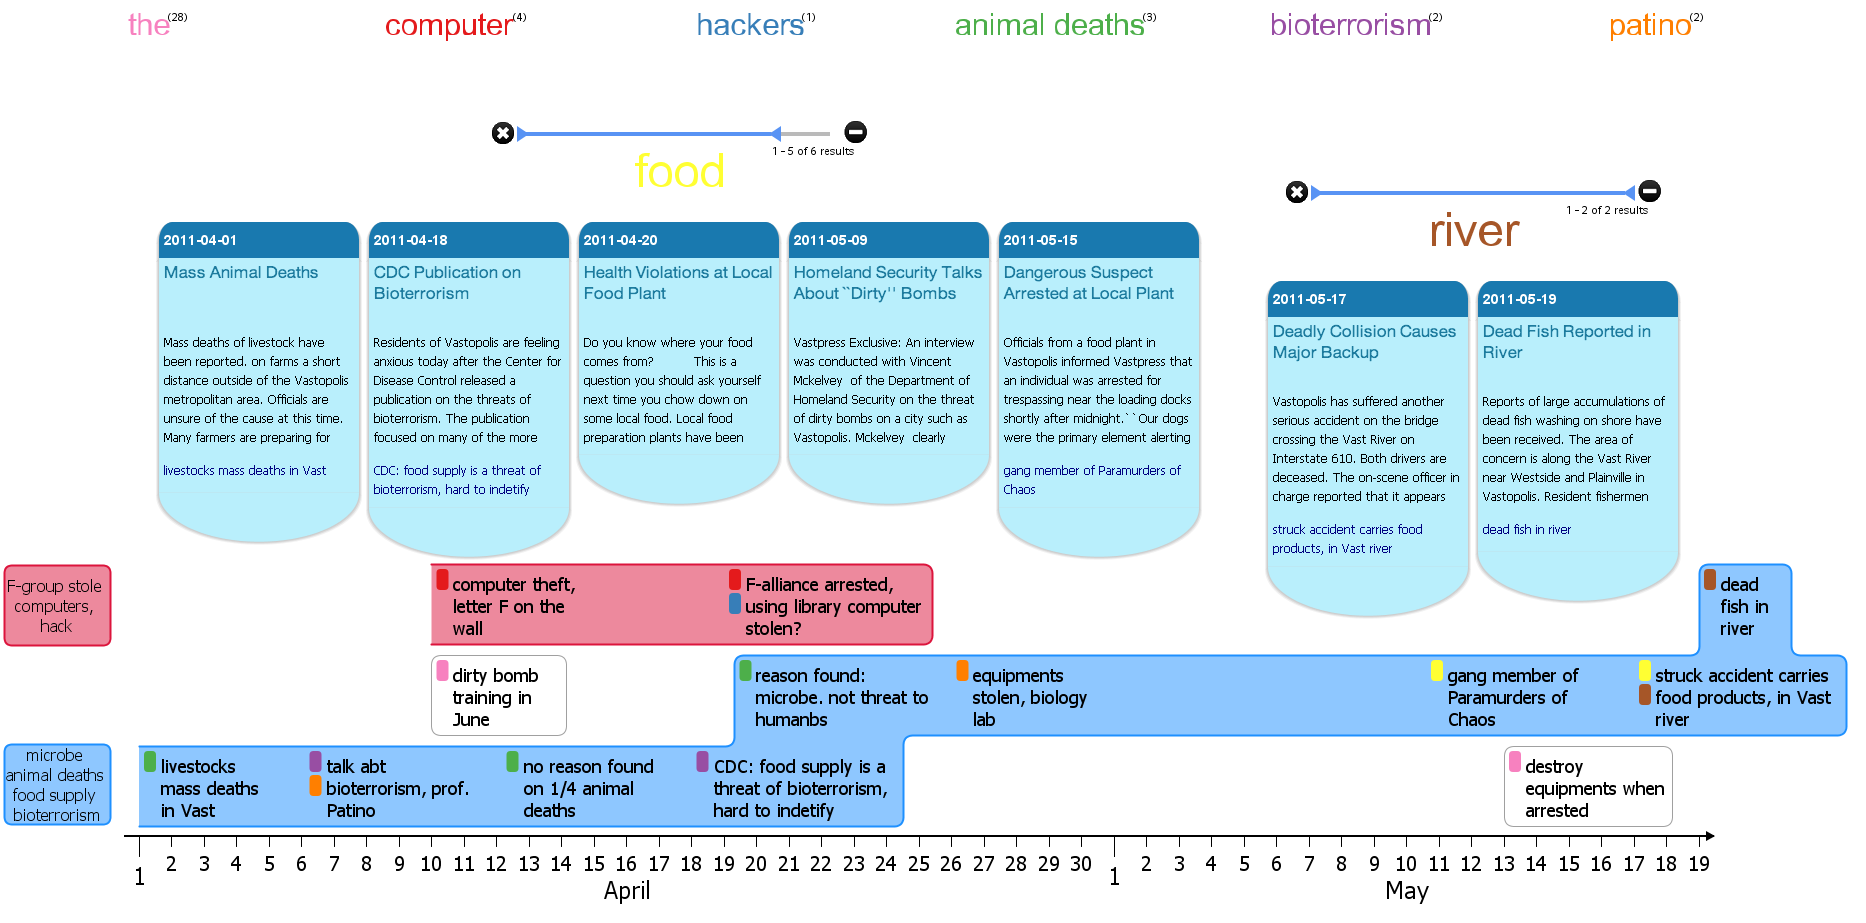
\includegraphics[width=\linewidth]{evaluation}
	\caption{Final screen of participant \textbf{P2}. Top: a trail of his keyword searches, collapsed after being read. Middle: search results in index-card metaphor. Bottom: two schemas containing notes as supporting evidence of criminal activities he found.}
	\label{fig:evaluation}
\end{figure*}

\paragraph{Participant 3}
\textbf{P3} searched for a few keywords related to criminal activities before examining the search results such as ``bomb'', ``terrorism'', ``money'' and ``hack''. He took and group notes about ``money laundering'' together (\emph{connect data and a frame}). Then, he read articles from ``terrorism'' search results. He followed the article content to search for relevant information such as ``Paramurderers of Chaos'' -- a terrorist group. During further investigation, similar to \textbf{P2}, he also combined two groups of notes -- ``Paramurderers of Chaos'' and ``food supply'' -- together when discovering evidence linking the two groups (\emph{merge frames}). When presenting his findings, he shared that SchemaLine prompted him to look for missing information. ``I noticed the gap between these two events [pointing to the timeline]; then I knew I probably missed something there'' (\emph{question the frame}). \textbf{P3} found the ``food poisoning'' case with 6/13 correct pieces of evidence, and a perfect 3/3 pieces of evidence in the ``money laundering'' case. 

\paragraph{Discussion}
% All take notes, build schemas
Three participants applied different sensemaking strategies. \textbf{P1} started with a potential search keyword for criminal activities and kept following the search results. \textbf{P2} initially scanned the titles of all documents to have an overview of the dataset. \textbf{P3} planned ahead what he wanted to search for and sequentially executed it. However, all of them extensively took notes and constructed explanatory frames from them. These frames presented various forms: a concept (bioterrorism), a criminal activity (dirty bomb), a person (Prof. Patino) and a group of people (Paramurderers of Chaos). All participants also employed a variety of sensemaking activities described in the Data--Frame model, supported through fluid interaction in SchemaLine: connect data and a frame, elaborate the frame, question the frame preserve the frame and merge frames.

% temporal sensemaking
All participants appreciated the automatic addition of analyst notes to SchemaLine. \textbf{P1} thought that he would have a problem if the system did not support that: ``I can remember what happened but it was difficult to remember when they happened''. They found that the chronological order of events provides cues to them to construct the story lines. \textbf{P2} shared that he read the news about the robbery at Vastopolis university and the Prof. Patino's talk about bioterrorism. However, he did not have any insight at that time. When looking at his two notes on the timeline, he thought that the extremely expensive equipment in Prof. Patino's lab could be the reason of the robbery. 

% intuitive interface & presentation
All participants commented that the interaction between data and frame was very intuitive. \textbf{P1} said ``I think I don't even need training and still can figure out how it works''. \textbf{P3} appreciated the transition effect when adding or removing notes because ``it helped me to understand what is going on''. All participants were confident while presenting their analyses. \textbf{P3} even opened the original document (double-clicking on the note) several times to highlight the relevant text. He said that the connection between the note and the containing document enabled him to quickly find the information source when needed.
%\section{Conclusion and Future Work}
\label{sec:conclusion}

In this paper, we introduced a new timeline visualization, SchemaLine, which is designed to support sensemaking. More specifically, it facilitates the schematization process in the Pirolli-Card model and targets all sensemaking activities in the Data-Frame model. The SchemaLine layout algorithm produces simple, compact, but aesthetically pleasing timeline visualizations. It replaces menu and buttons with fluid user interactions to perform all necessary tasks, and can be integrated within larger visual analytic systems. Our preliminary evaluation suggests that the design of SchemaLine is supportive of sensemaking tasks. It was clearly a helpful aid to users in analysis of the scenario, as evidenced by their usage patterns and feedback. 

As future work, a more formal evaluation would be beneficial -- perhaps even following integration of SchemaLine into a number of different systems, to allow the specific effect to be separated from the rest of the system. In terms of design of the SchemaLine itself, there are a number of improvements that could be added. Shared events between frames could be better visualized (at present, the event is simply duplicated). There are also obvious issues with scalability: while the timeline will scale comparatively well with number of events, it will scale badly with number of frames, since the set of effective qualitative colors is quite small. Other cues such as texture or line style may help with this problem, but to discover this will require further experimentation.